\begin{frame}
\frametitle{Significance de l'observation}

\begin{small}
\begin{maliste}
\item Approche par d\'efaut : hybride
\begin{itemize}
\item[$\rightarrow$] incertitudes syst\'ematiques : interpolation/extrapolation mclimit
\item[$\rightarrow$] incertitudes statistiques : \english{prior} gaussien
\end{itemize}
\end{maliste}
\end{small}

\vspace*{-0.42cm}
\begin{columns}
\begin{column}{0.5\textwidth}
\begin{figure}[!htb]
\begin{center}
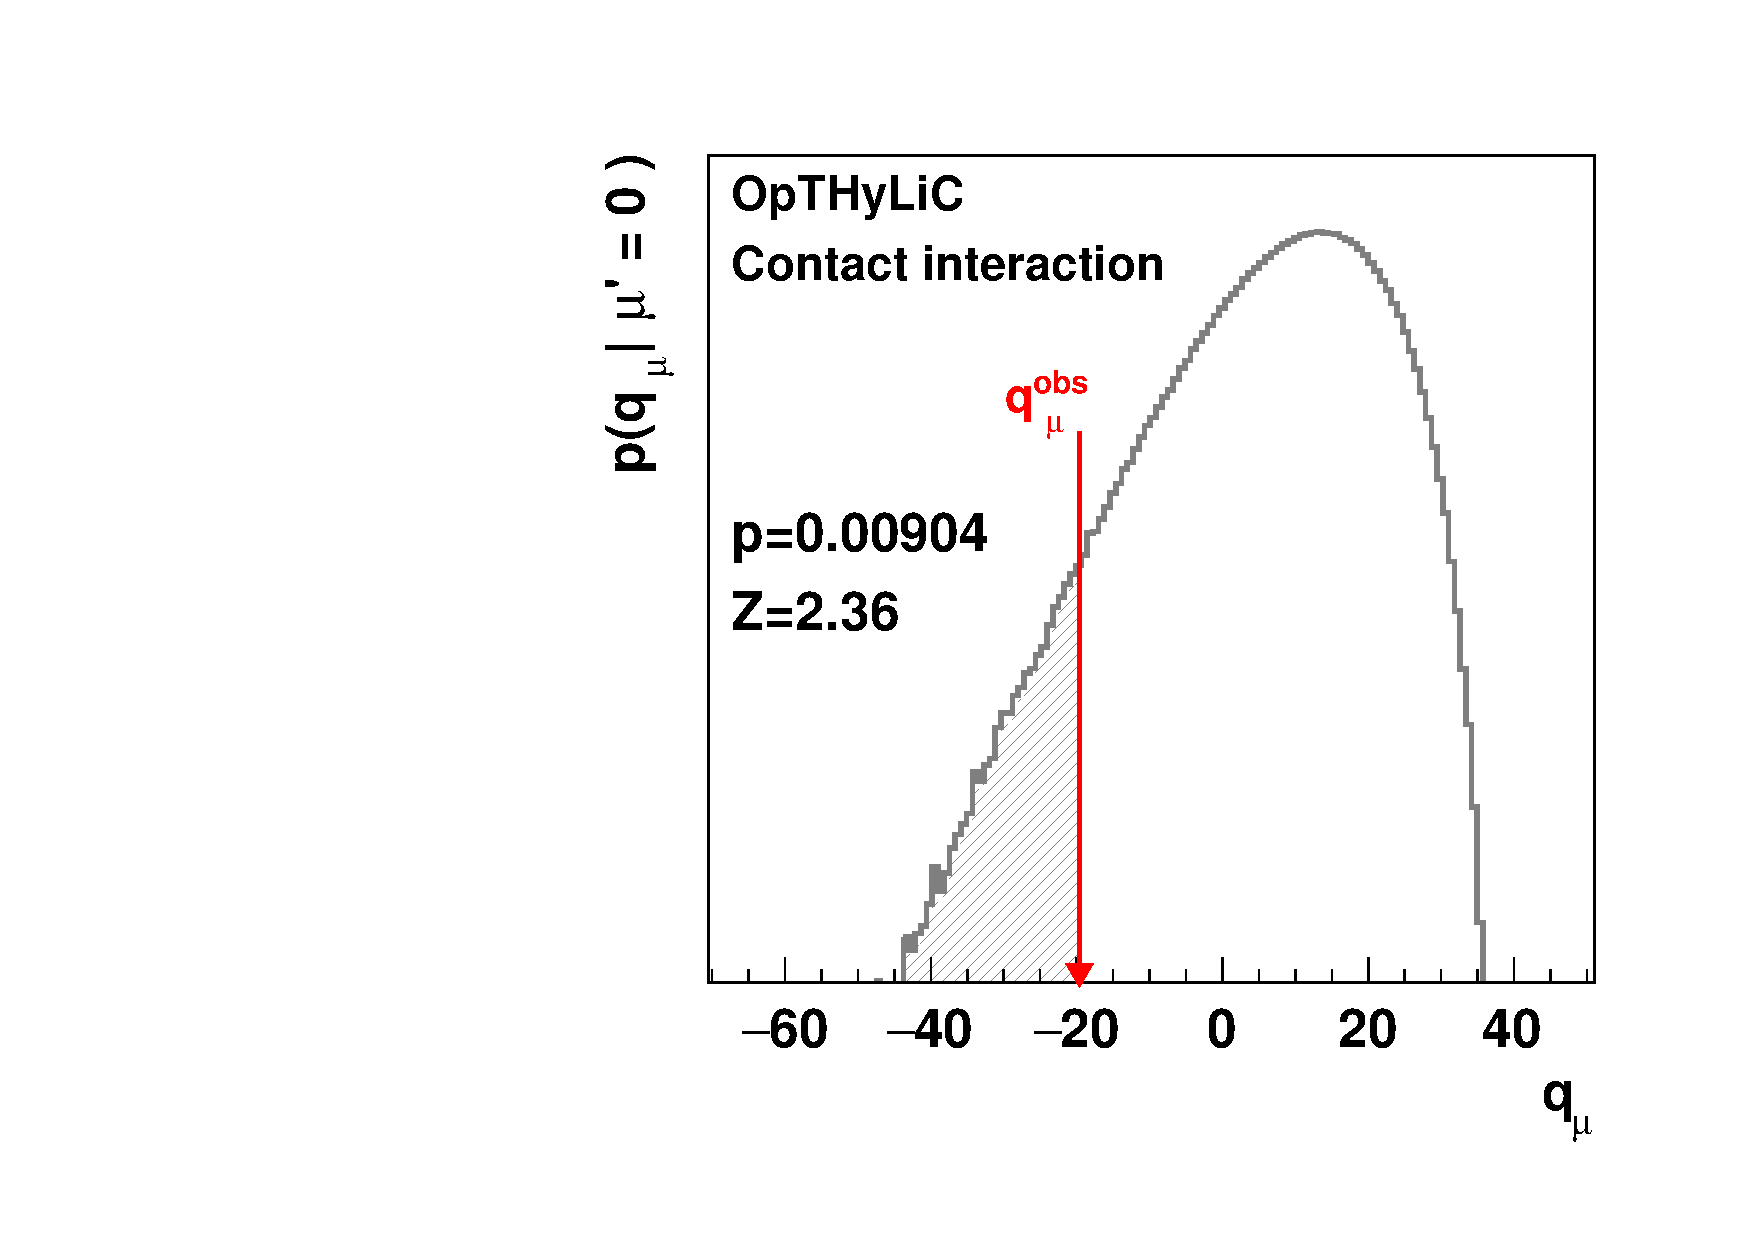
\includegraphics[width=0.65\linewidth]{Figures/FourTops/significanceContactInteractionMcLimitNormal.pdf}\\
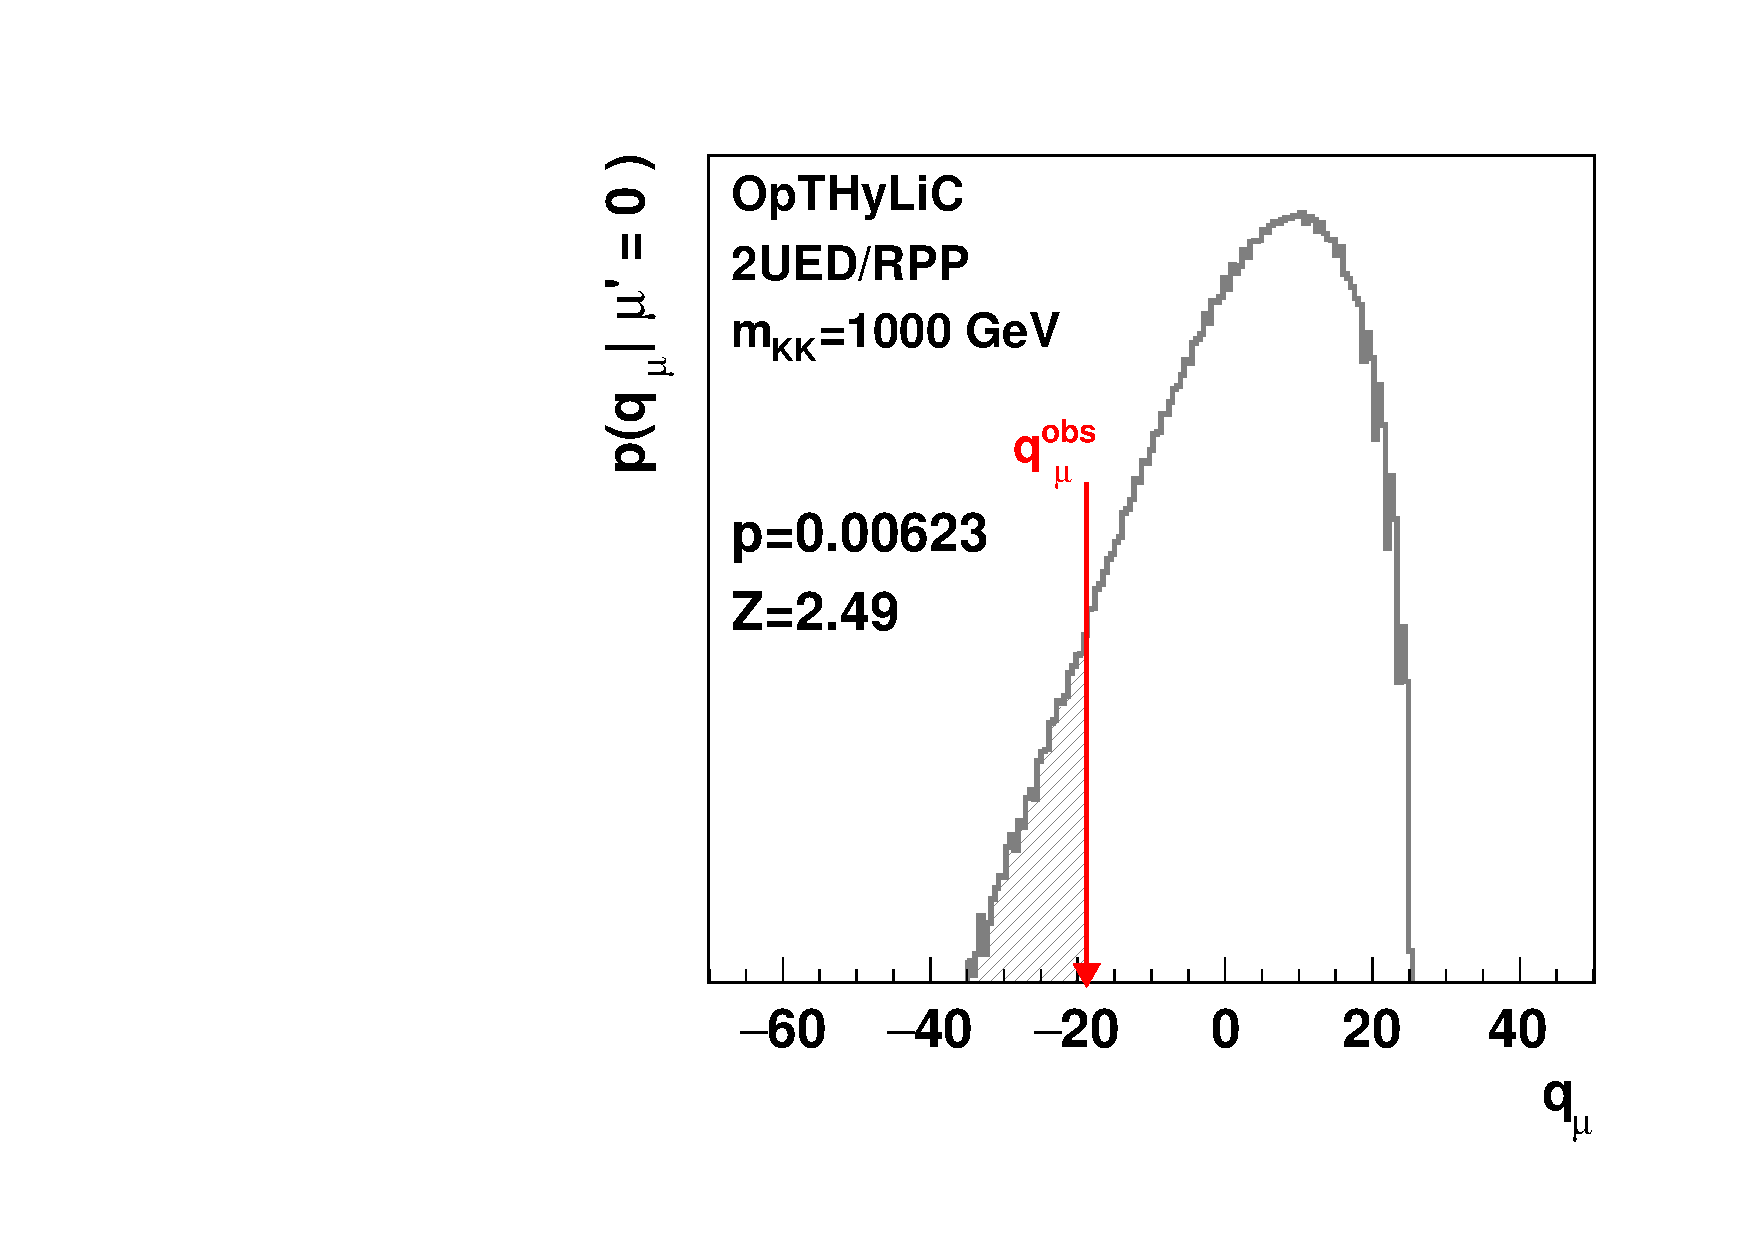
\includegraphics[width=0.65\linewidth]{Figures/FourTops/significance2UEDRPPMkk1000McLimitNormal.pdf}
\end{center}
\end{figure}
\end{column}
\begin{column}{0.5\textwidth}
\begin{varblock}[4cm]{}
\[p = \sum\limits_{-\infty}^{\qmuobs} P\left(\qmu|\mu'=0\right)\]
\[Z=\Phi^{-1}\left(1-p\right)\]
\end{varblock}

\begin{center}
\hspace*{-2cm}
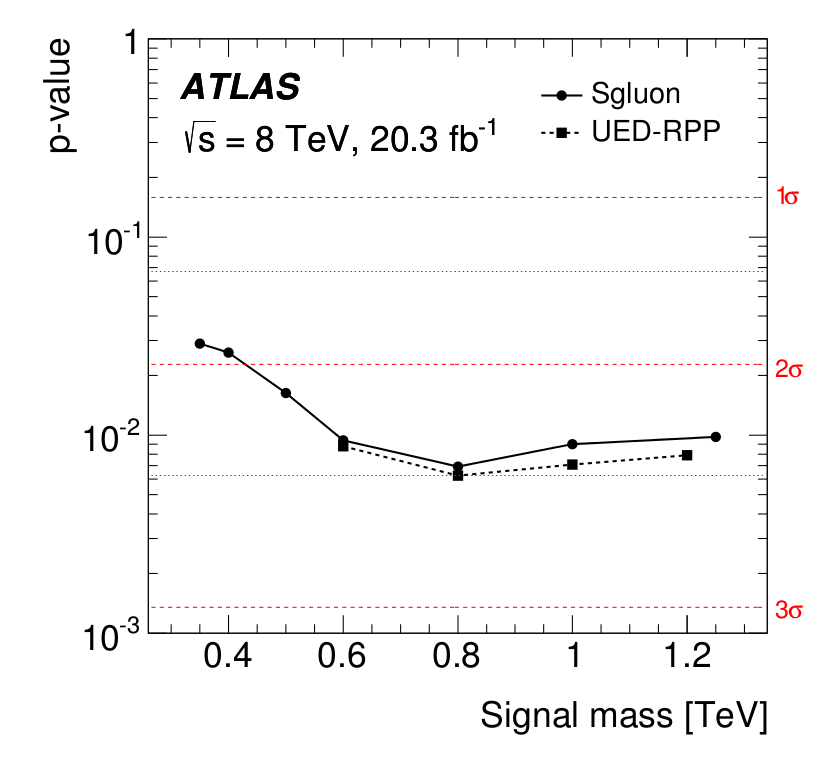
\includegraphics[width=0.9\linewidth]{Figures/FourTops/significanceVssignalmass.png}
\end{center}
\end{column}
\end{columns}
\end{frame}

\begin{frame}
\frametitle{Limites d'exclusion}

\begin{small}
\begin{maliste}
%\item R\'esultats publi\'es (JHEP 10 (2015) 150) : approche hybride
\item R\'esultats avec approche hybride par d\'efaut :
\end{maliste}

\begin{figure}[!htb]
\begin{center}
\hspace*{-1cm}
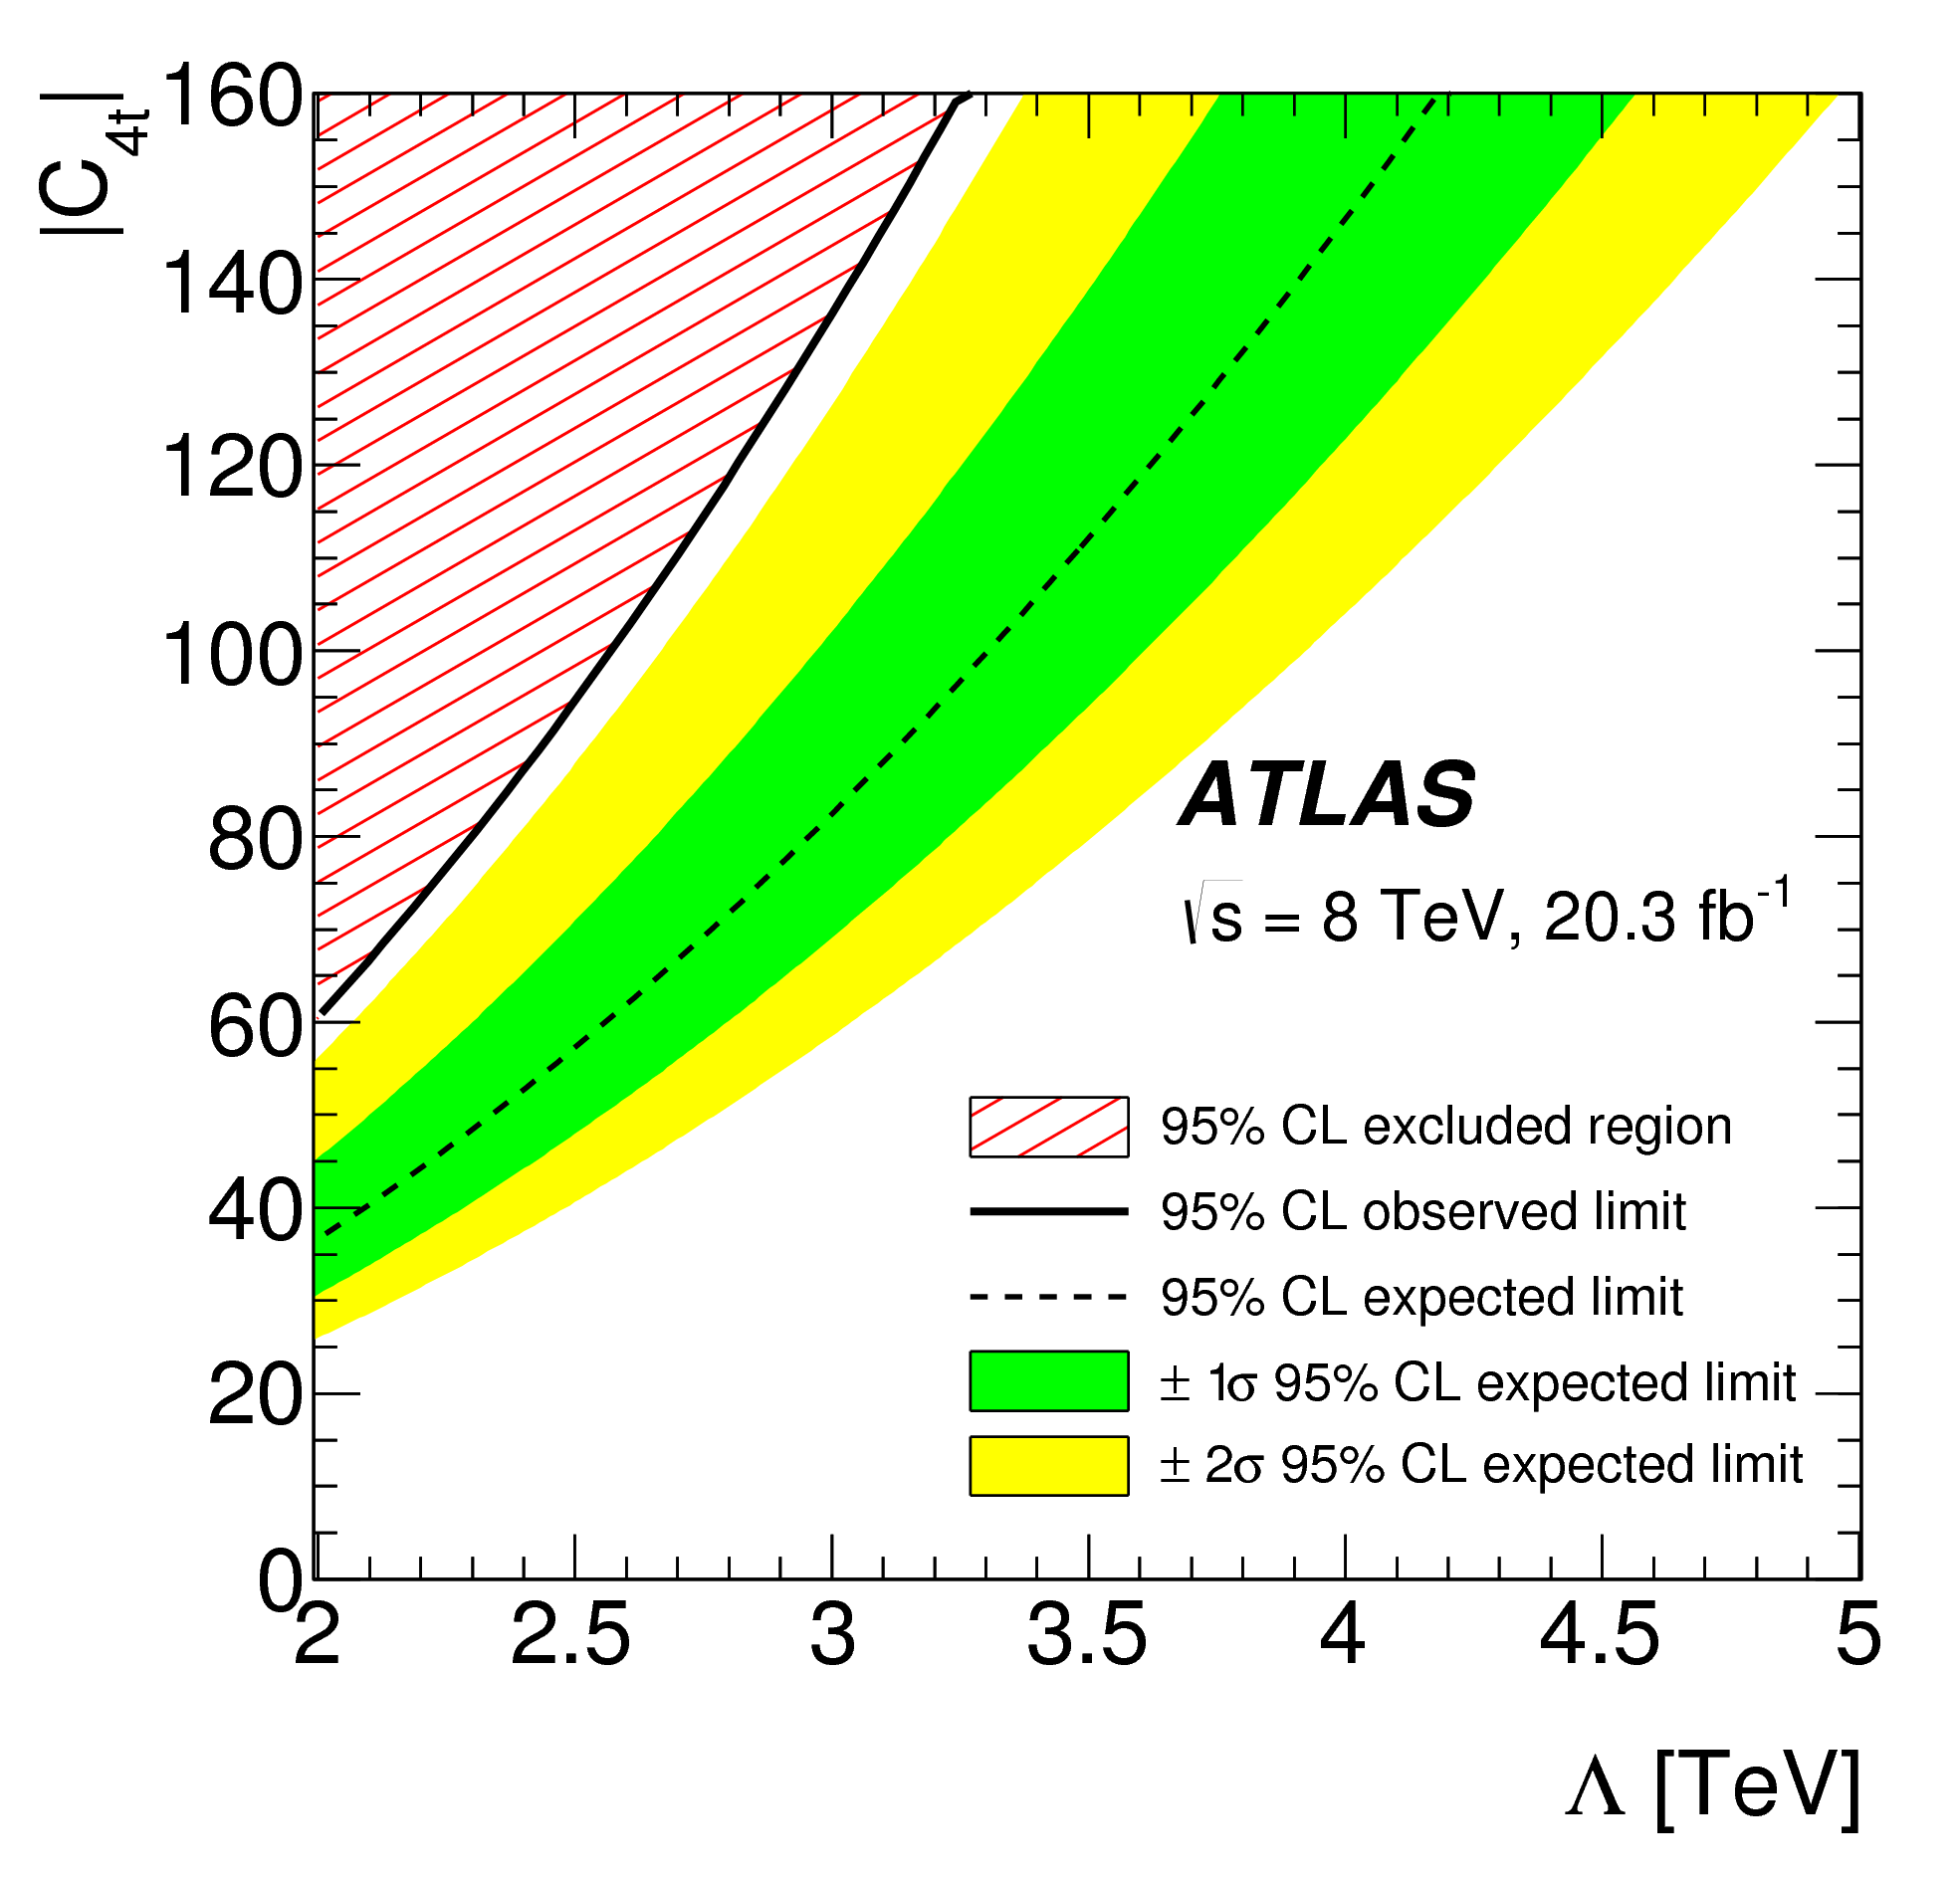
\includegraphics[width=0.45\textwidth]{Figures/FourTops/fig_11a.png}
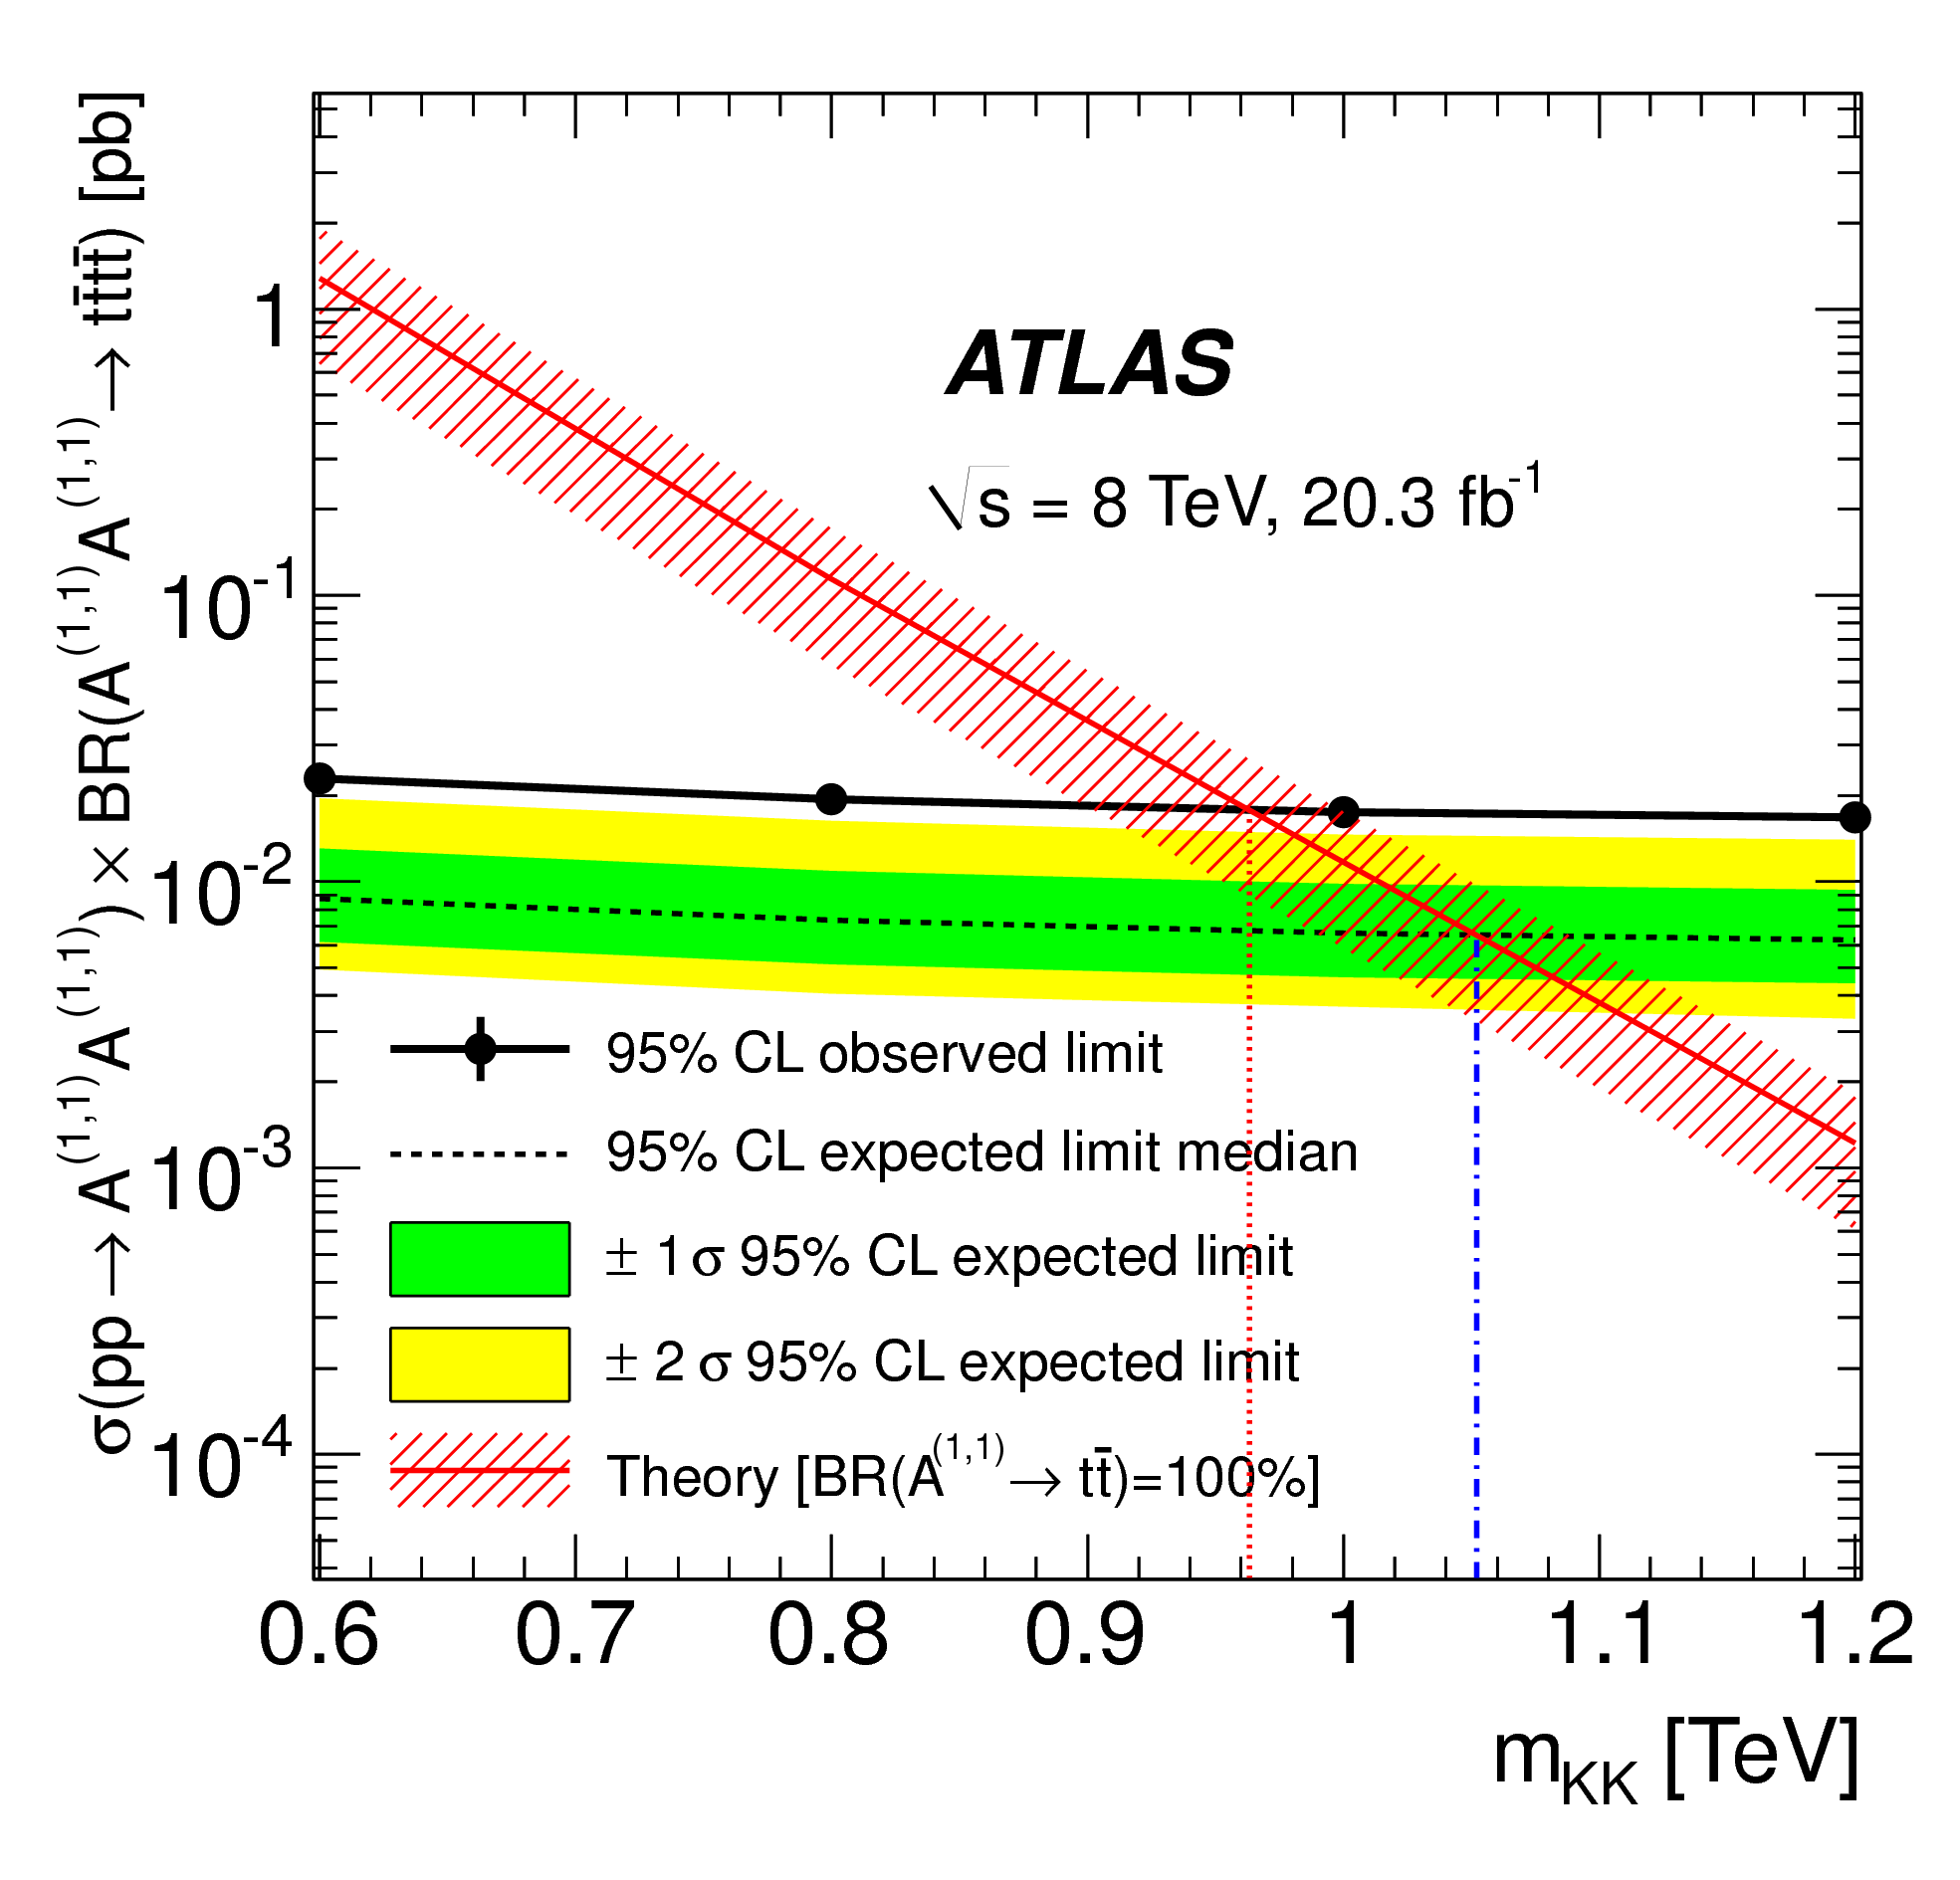
\includegraphics[width=0.45\textwidth]{Figures/FourTops/fig_11c.png}
\end{center}
\end{figure}
\begin{maliste}
\item Modèle standard : $\sigma < 70~(27)$~fb observed (expected)
\vspace*{0.1cm}
\item Interaction de contact : $\sigma < 61~(22)$~fb observed (expected) \\
\begin{center}
$\Rightarrow$ $\frac{C}{\Lambda^2} < 15,1$~TeV$^{-2}$
\end{center}
\vspace*{0.1cm}
\item 2UED/RPP : $m_{KK}>0,96~(1,05)$~TeV pour $\xi=1$
%\item Dans 2 cas : excès $>2\sigma$
\end{maliste}
\end{small}
\end{frame}

\begin{frame}
\frametitle{R\'e-interprétation 2UED/RPP}

\begin{small}
\begin{maliste}
\item Cas $\xi=1$ exclu \\
\begin{center}
$\rightarrow$ R\'e-interpr\'etation r\'esultat $\xi=1$ aux cas $\xi\neq 1$
\end{center}
\vspace*{0.2cm}
\item Phénoménologie étage $(1,1)$ ne dépend au $1^\text{er}$ ordre que de 
\begin{columns}
\begin{column}{0.7\textwidth}
\begin{small}
\[\text{masse}_{(1,1)}\simeq\sqrt{\frac{1}{R_4^2}+\frac{1}{R_5^2}}=m_{KK}\sqrt{1+\xi^2}\]
\end{small}
\end{column}
\begin{column}{0.3\textwidth}
%\hspace*{-1cm}
\begin{varblock}[3cm]{}
\[\xi=\frac{R_4}{R_5},\quad m_{KK}=\frac{1}{R_4}\]
\end{varblock}
\end{column}
\end{columns}
\end{maliste}
\end{small}

\begin{figure}[!htb]
\begin{center}
\hspace*{-1cm}
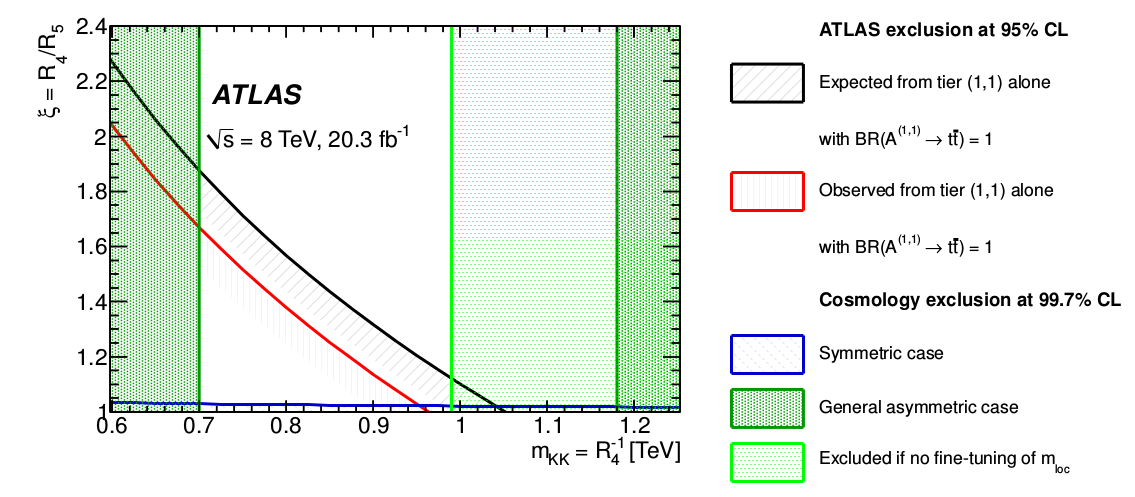
\includegraphics[width=0.85\textwidth]{Figures/FourTops/fig_12.png}
\end{center}
\end{figure}
\end{frame}

\begin{frame}
\frametitle{Interpr\'etation hybride vari\'ee}

\vspace*{-0.5cm}
\begin{center}
\begin{small}
\[
\hspace*{-0.2cm}
P\left(\{\nc\}|\textcolor{blue}{\mu}\right)=\displaystyle\int P\left(\{\nc\}|\textcolor{blue}{\mu},\textcolor{red}{\{\scc',\bci',\eta_j\}}\right)\times \textcolor{red}{\prod\limits_{c}f\left(\scc'\right)\prod\limits_{i}f\left(\bci'\right)\prod\limits_{j}g\left(\eta_j\right)}\textcolor{red}{\dd\scc'\dd\bci'\dd\eta_j}
\]
\end{small}
\end{center}
\vspace*{-0.5cm}
\begin{columns}
\begin{column}{0.7\textwidth}
\begin{footnotesize}
\begin{maliste}
\item Changement des distributions \prior~:
\begin{itemize}
\item Interp./extrap. incertitudes syst\'ematiques : 
\vspace*{-0.1cm}
\begin{center}
\textcolor{magenta}{mclimit $\rightarrow$ polynomiale + exponentielle}
\end{center}
\vspace*{0.1cm}
\item Incertitudes stat. : 
\vspace*{-0.1cm}
\begin{center}
\textcolor{magenta}{normal $\rightarrow$ gamma (prior hyperbolique)}
\end{center}
\end{itemize}
\vspace*{0.1cm}
\item Effet similaire pour \english{prior} log-normal
\end{maliste}
\end{footnotesize}
\end{column}
\begin{column}{0.3\textwidth}
\hspace*{0.5cm}
\vspace*{-0.5cm}
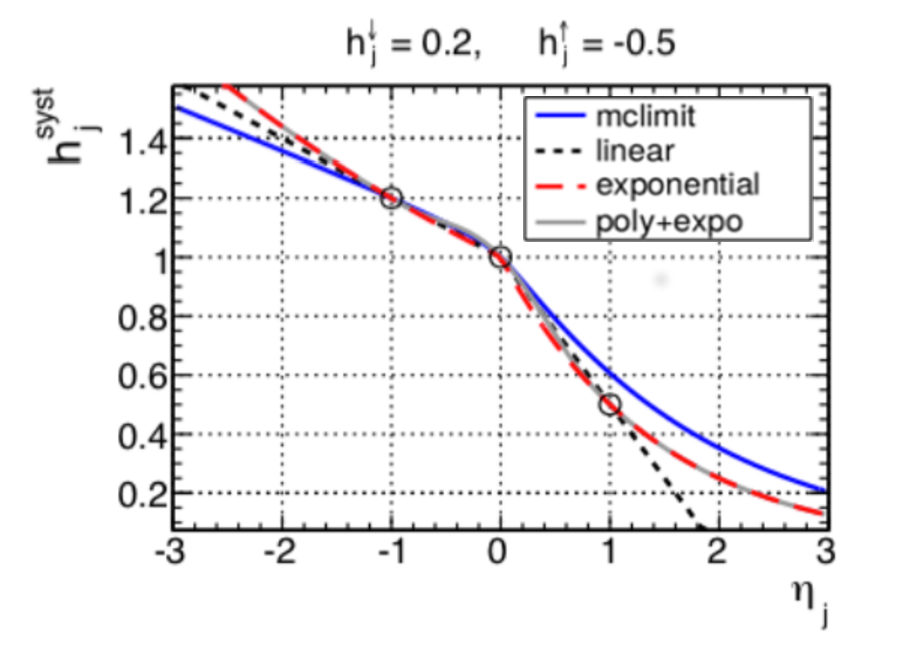
\includegraphics[width=0.99\textwidth]{Figures/Stat/cFunctionsInterExtrap_cropped3.pdf}\\
\vspace*{-0.3cm}
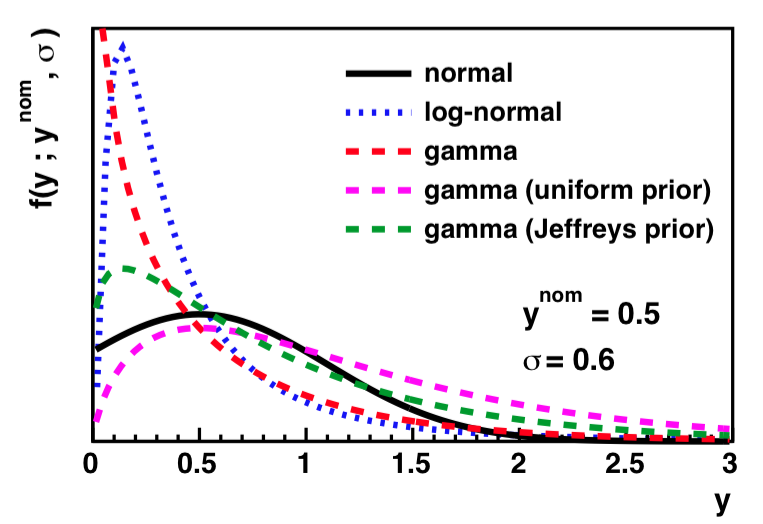
\includegraphics[width=0.9\textwidth]{Figures/Stat/plotNormalLogNGamma_cropped.png}
\end{column}
\end{columns}

%\vspace*{-0.8cm}
%\begin{center}
%\begin{figure}[!htb]
%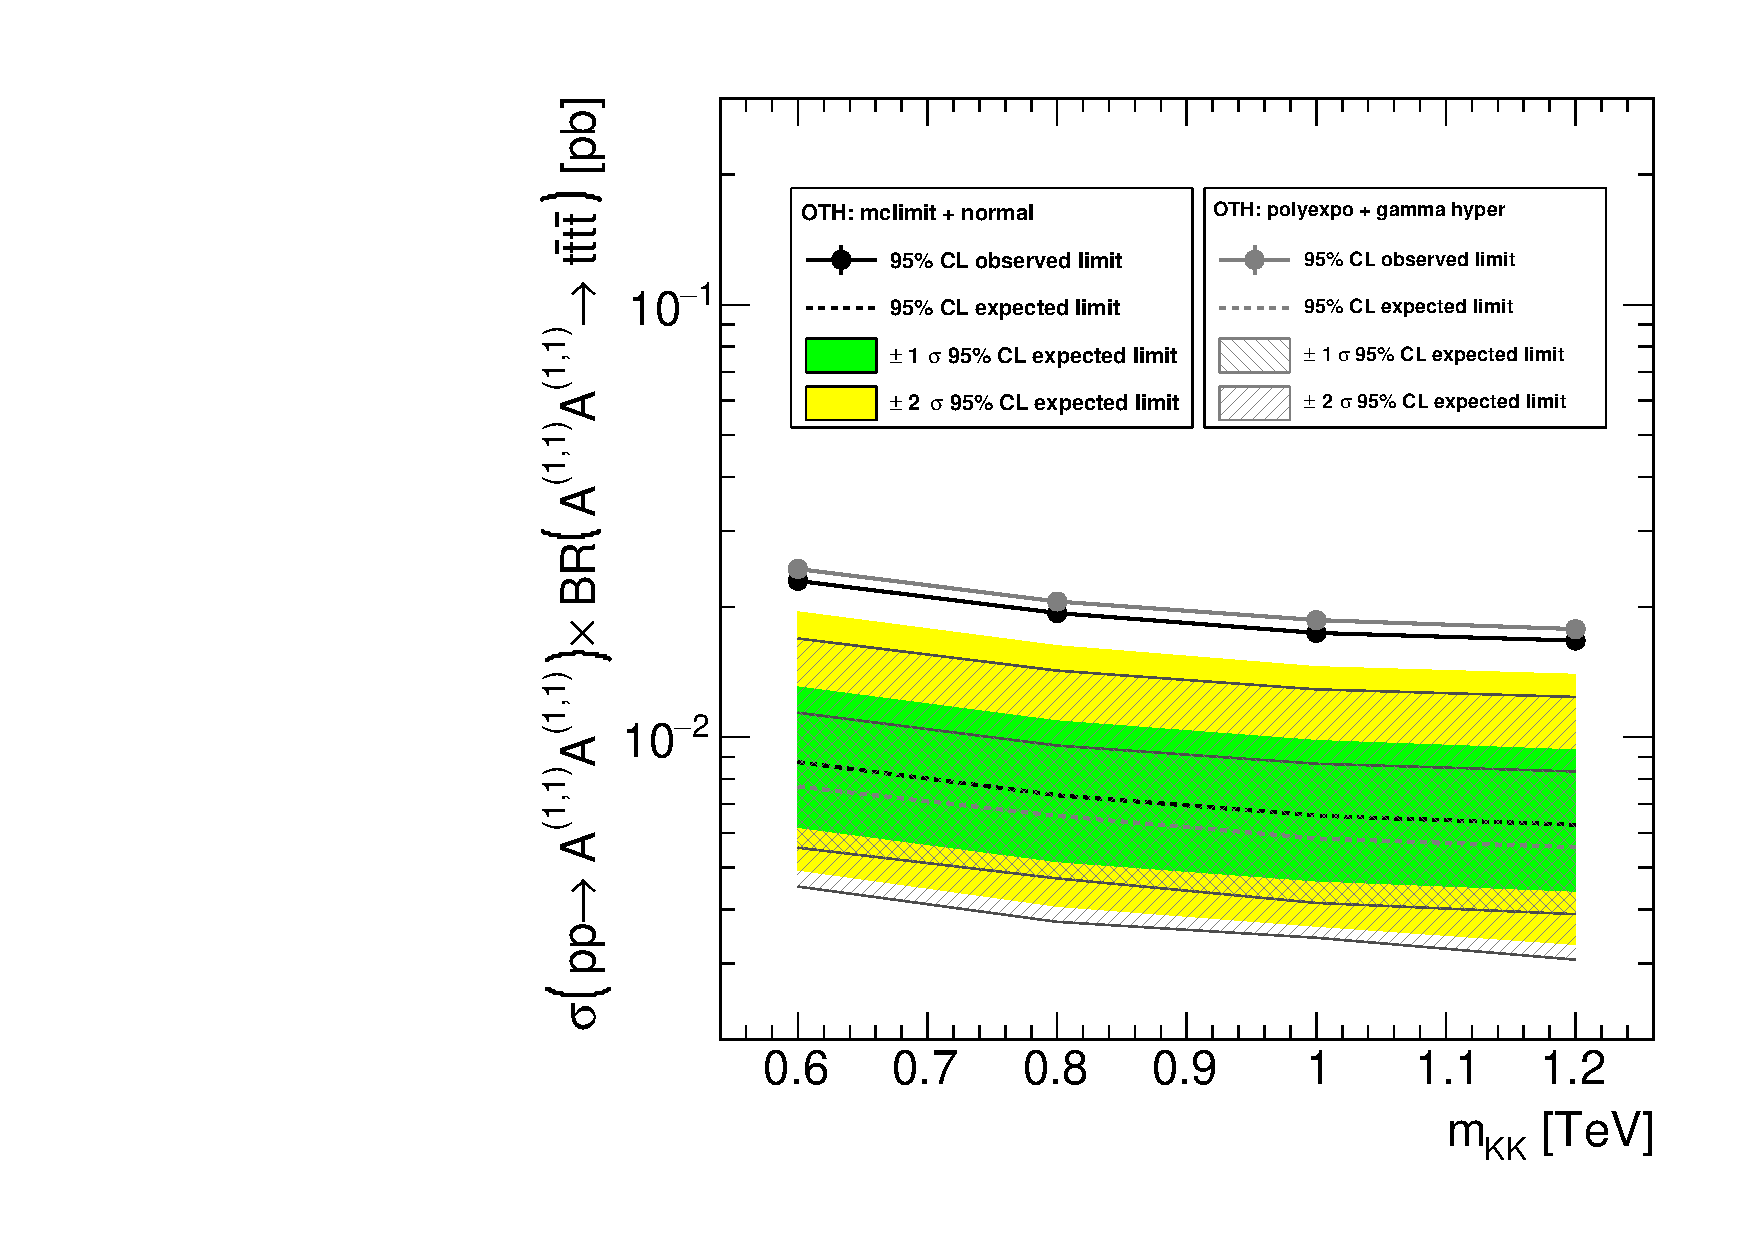
\includegraphics[width=0.35\textwidth]{Figures/FourTops/ExclusionPlot_RPPFullStat_McLimitVsOTHpolyexpo_gammahyper.pdf}
%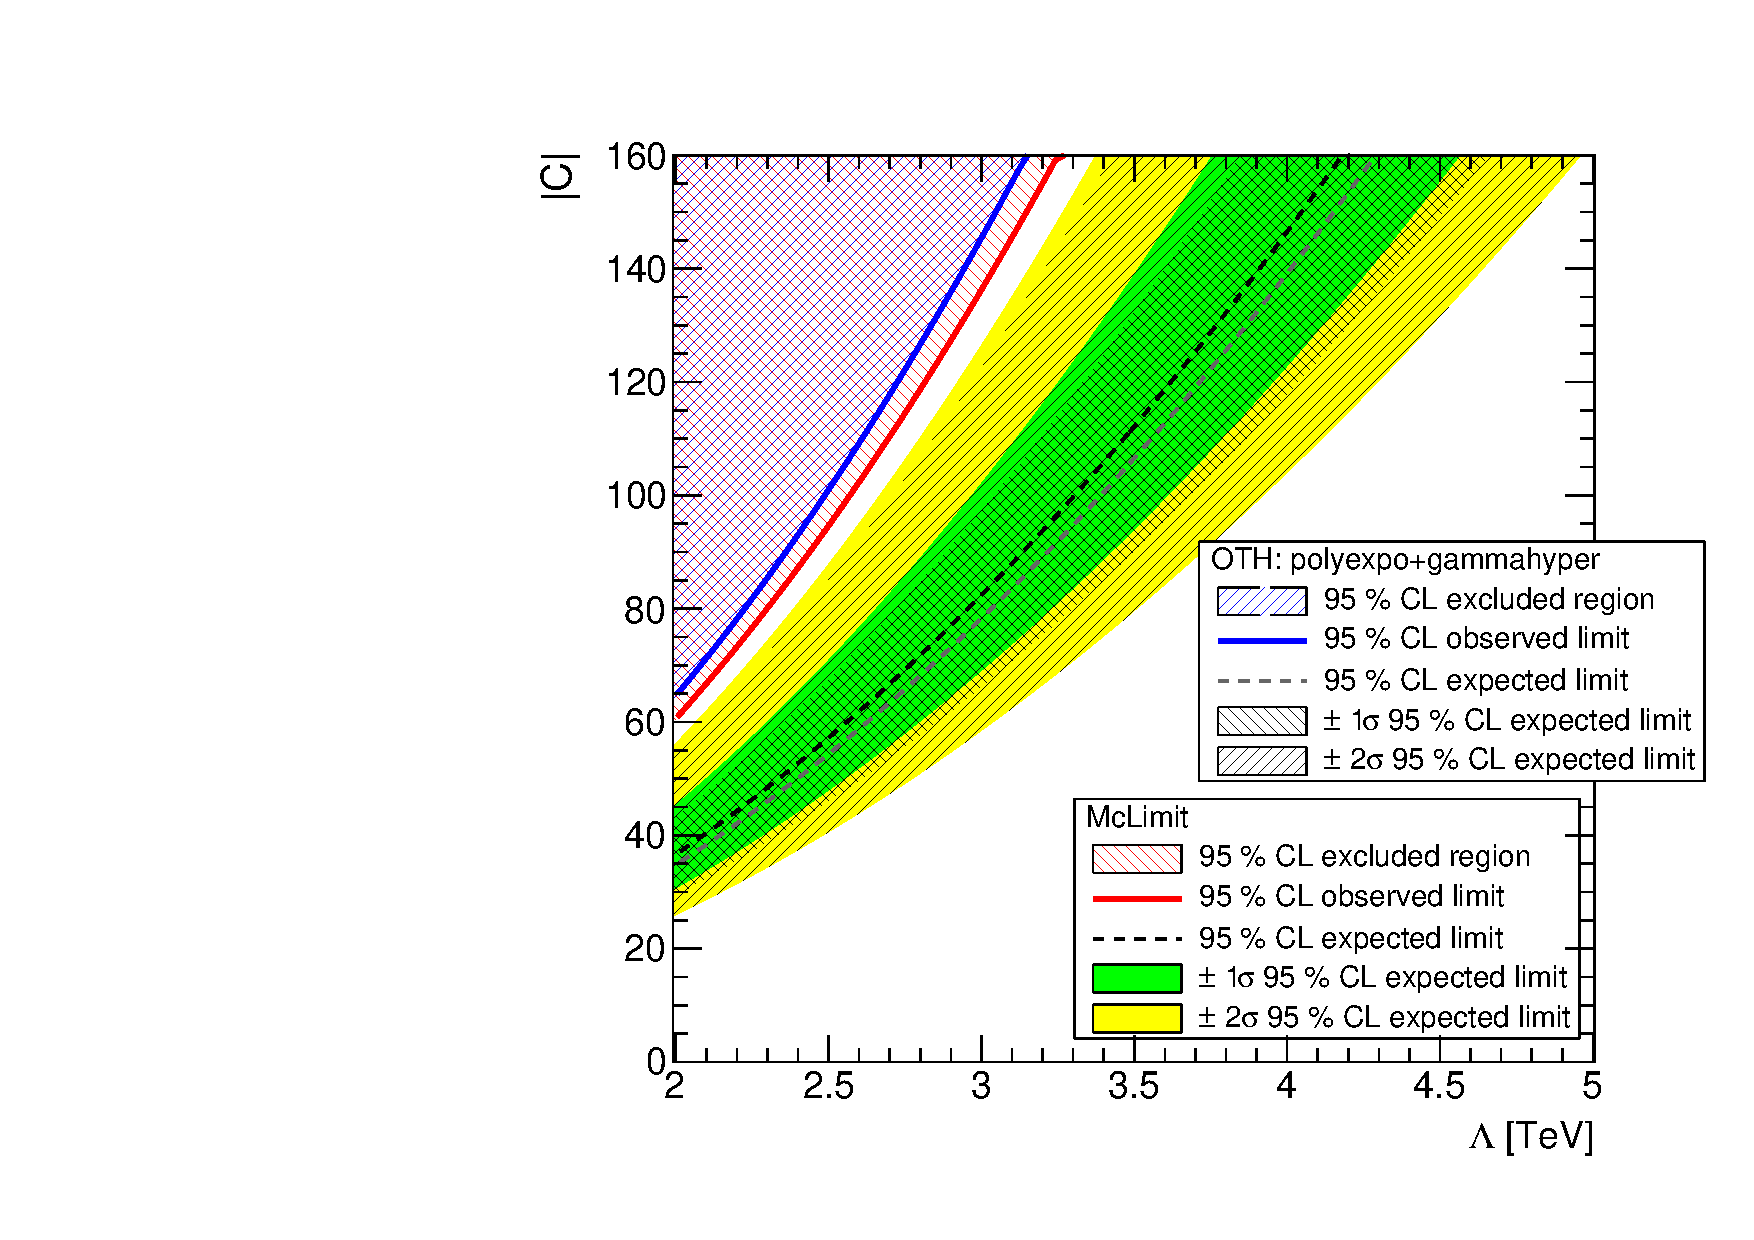
\includegraphics[width=.37\textwidth]{Figures/FourTops/CVsLambdaForContactInteractionMcLimitVsOTHpolyexpogammahyper.pdf}
%\vspace*{0.1cm}
%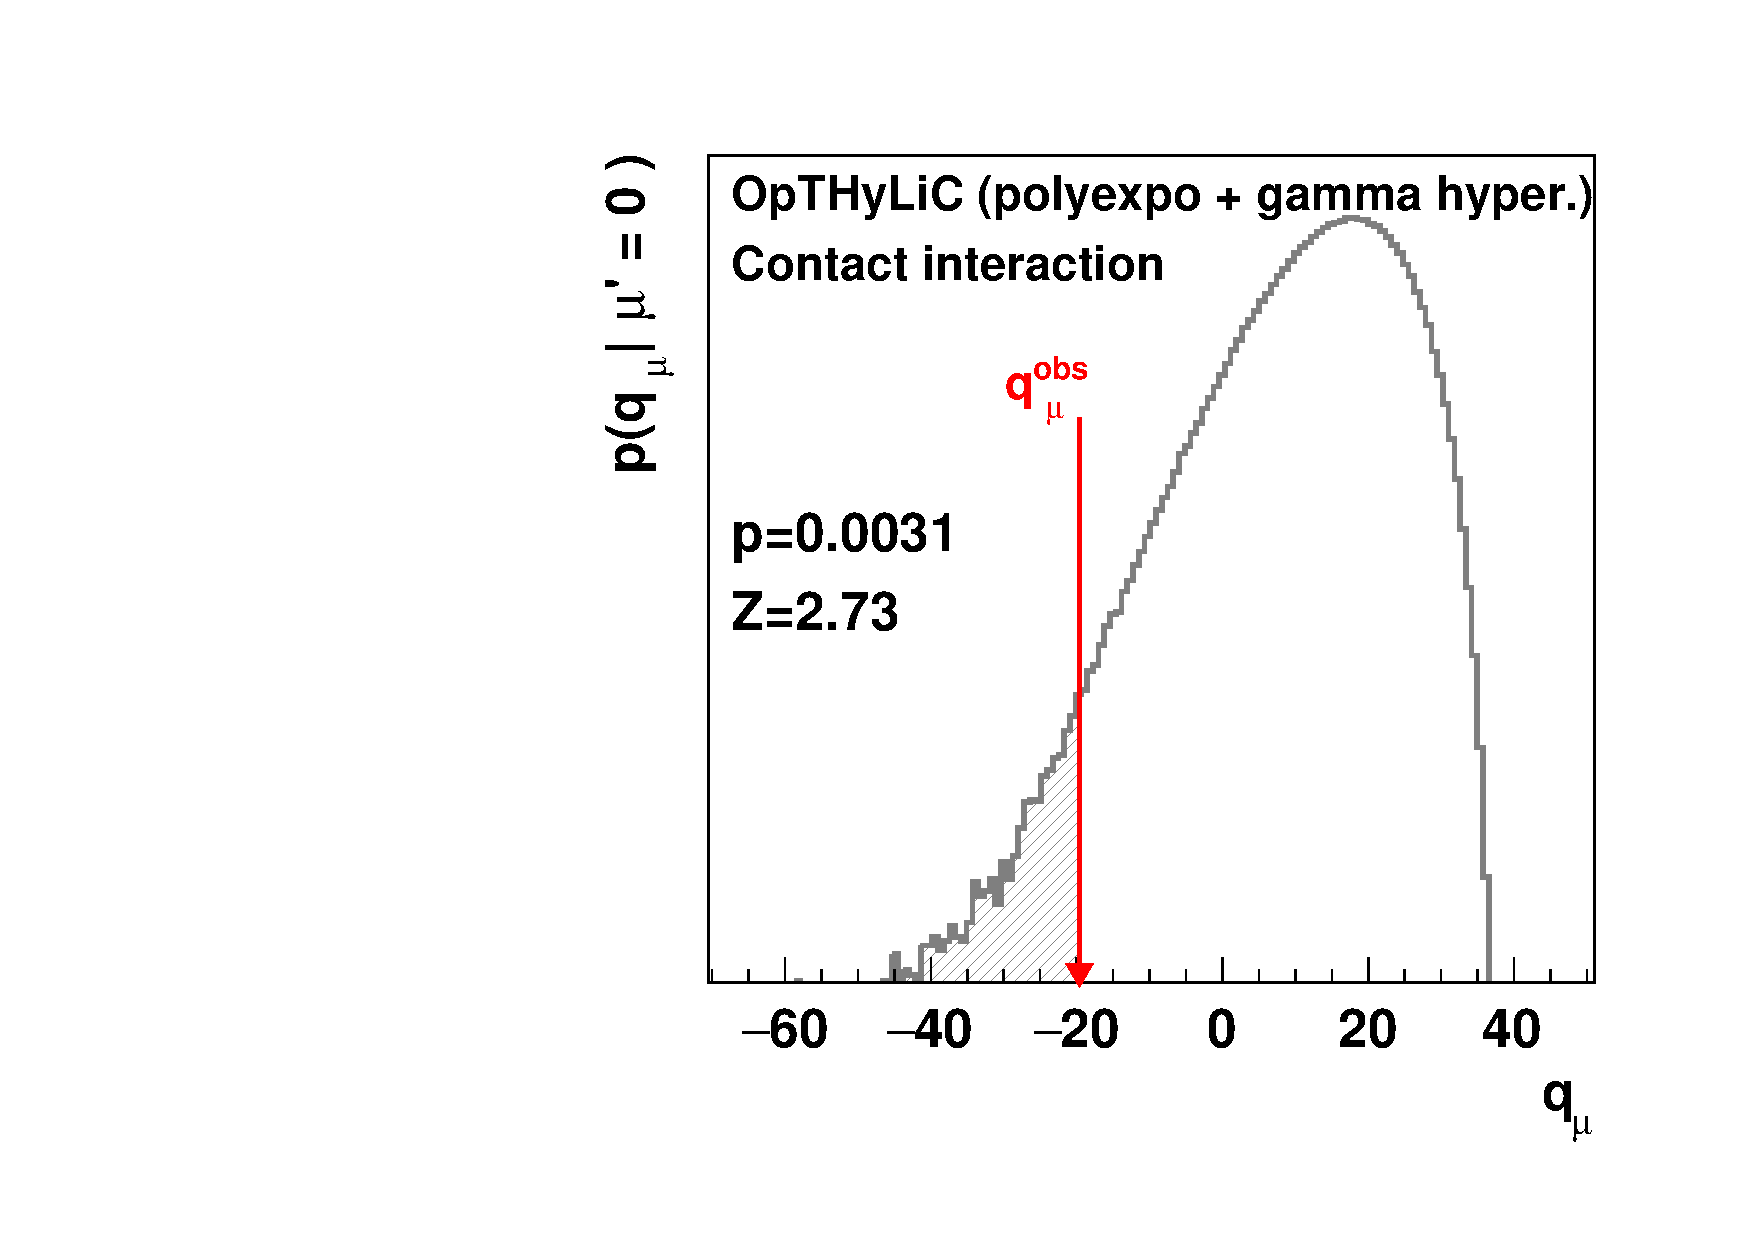
\includegraphics[width=.39\textwidth]{Figures/FourTops/significanceContactInteractionPolyExpoGammaHyper.pdf}
%\end{figure}

\begin{columns}
\begin{column}{0.7\textwidth}
\begin{center}
\vspace*{-1cm}
\begin{figure}[!htb]
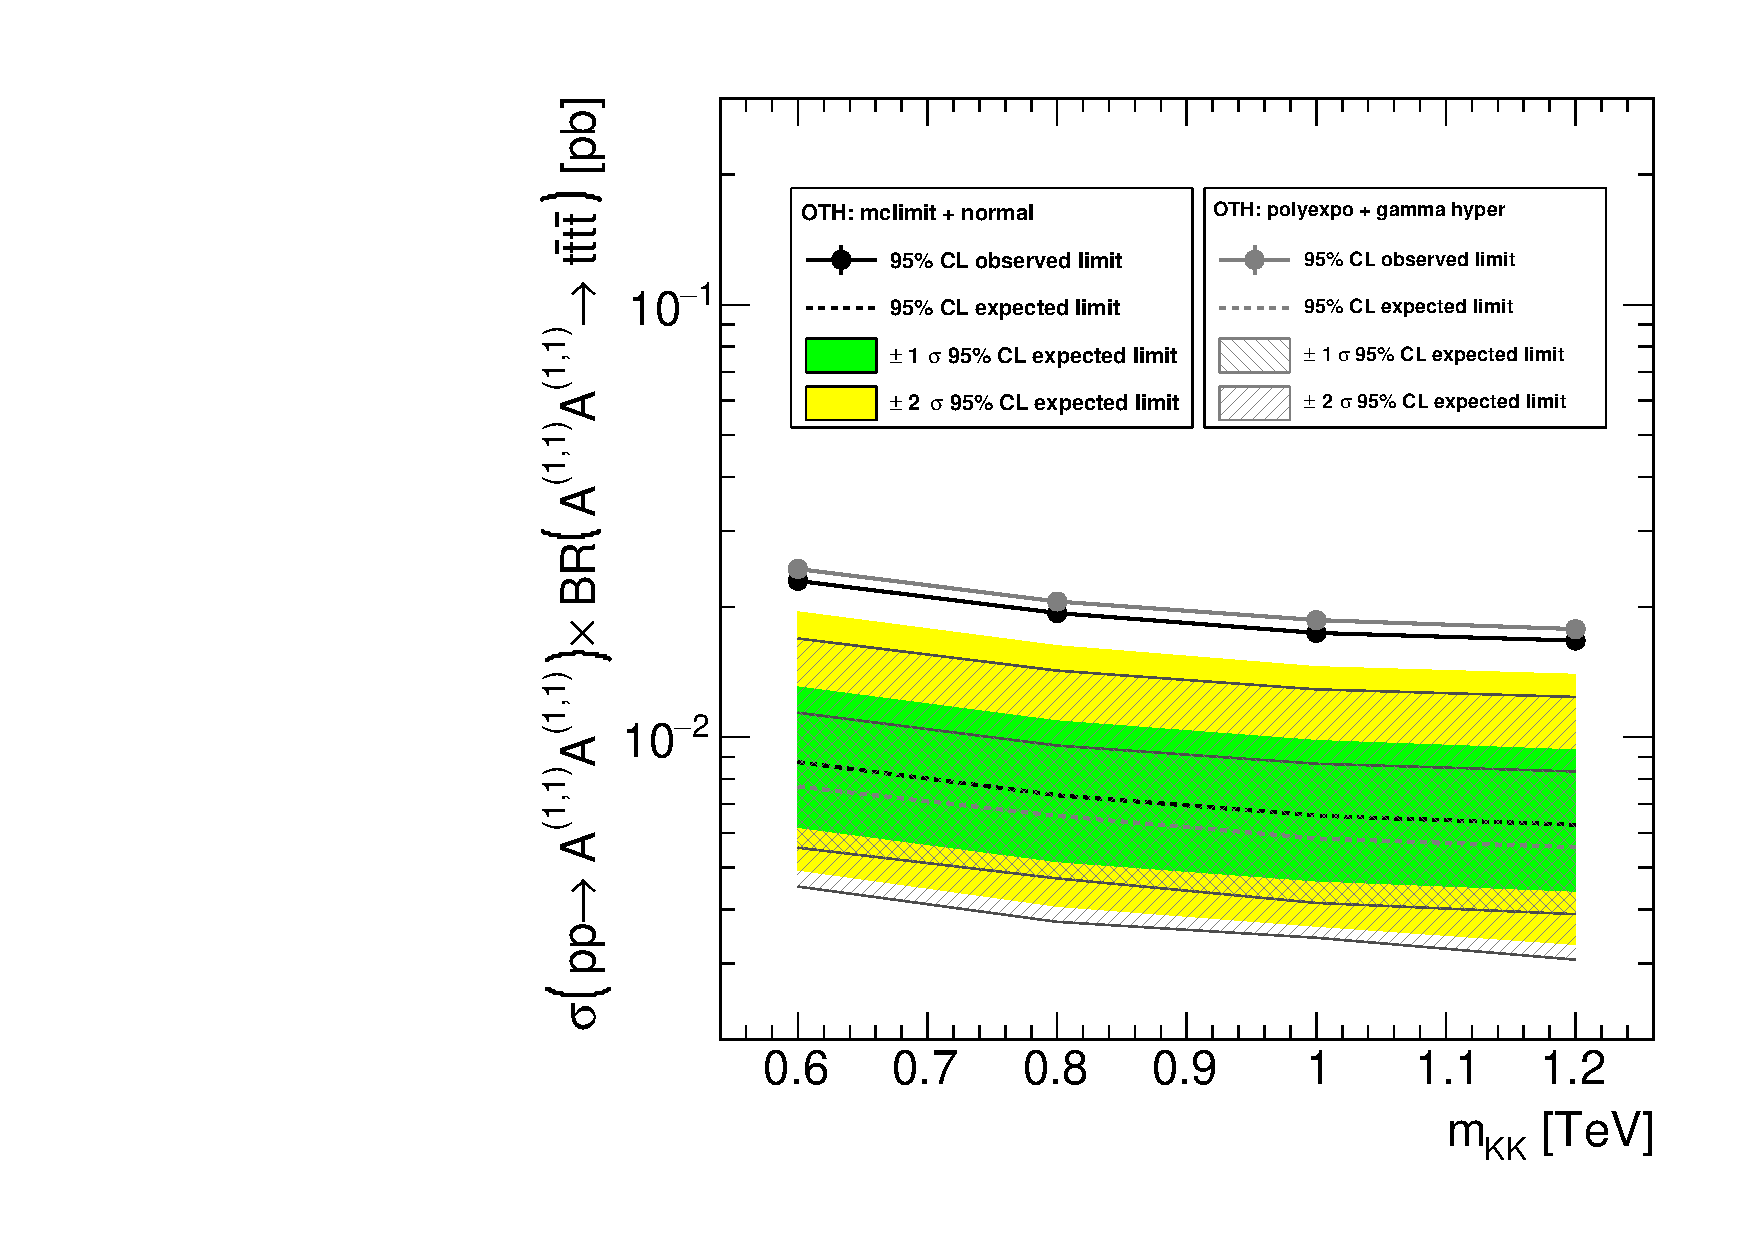
\includegraphics[width=0.45\textwidth]{Figures/FourTops/ExclusionPlot_RPPFullStat_McLimitVsOTHpolyexpo_gammahyper.pdf}
\hspace*{0.4cm}
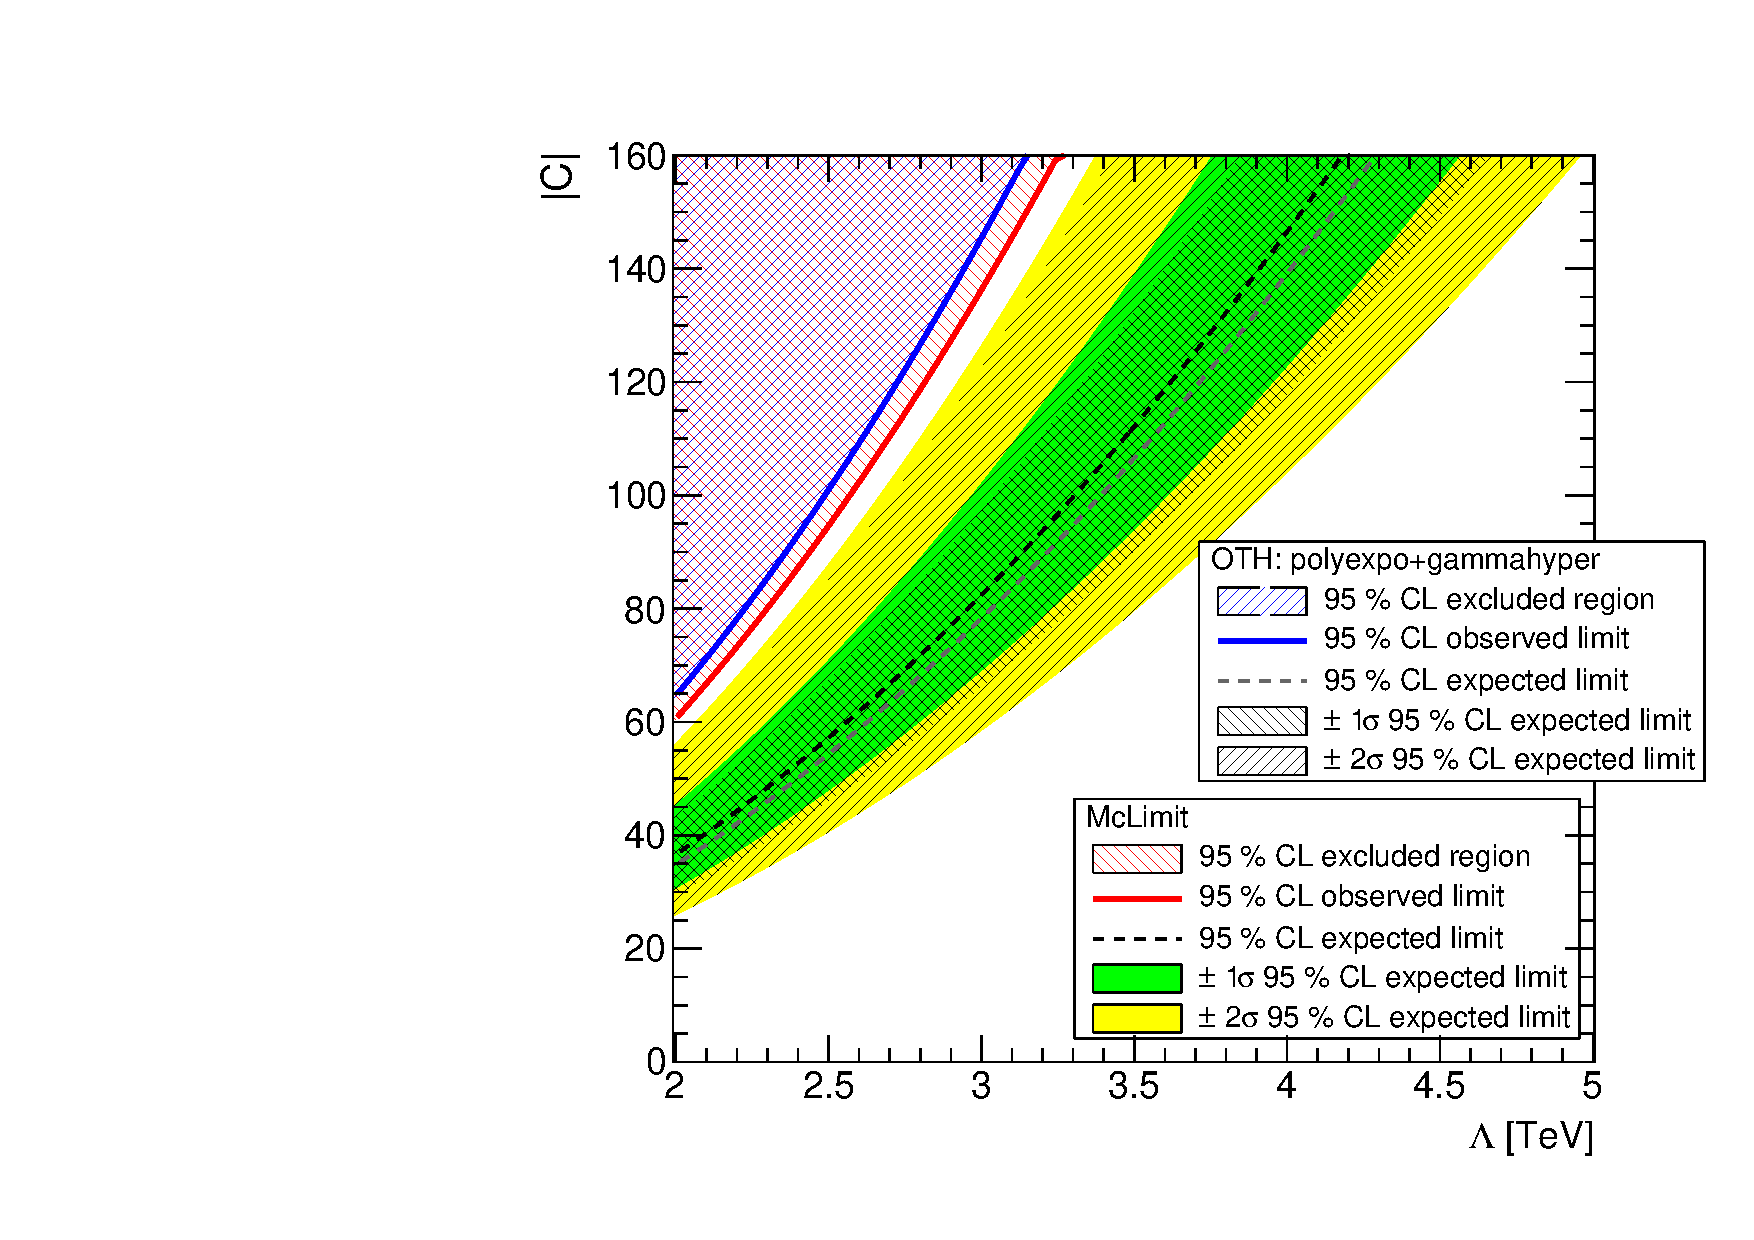
\includegraphics[width=.47\textwidth]{Figures/FourTops/CVsLambdaForContactInteractionMcLimitVsOTHpolyexpogammahyper.pdf}
\end{figure}
\end{center}
\end{column}
\begin{column}{0.3\textwidth}
\begin{center}
\begin{figure}[!htb]
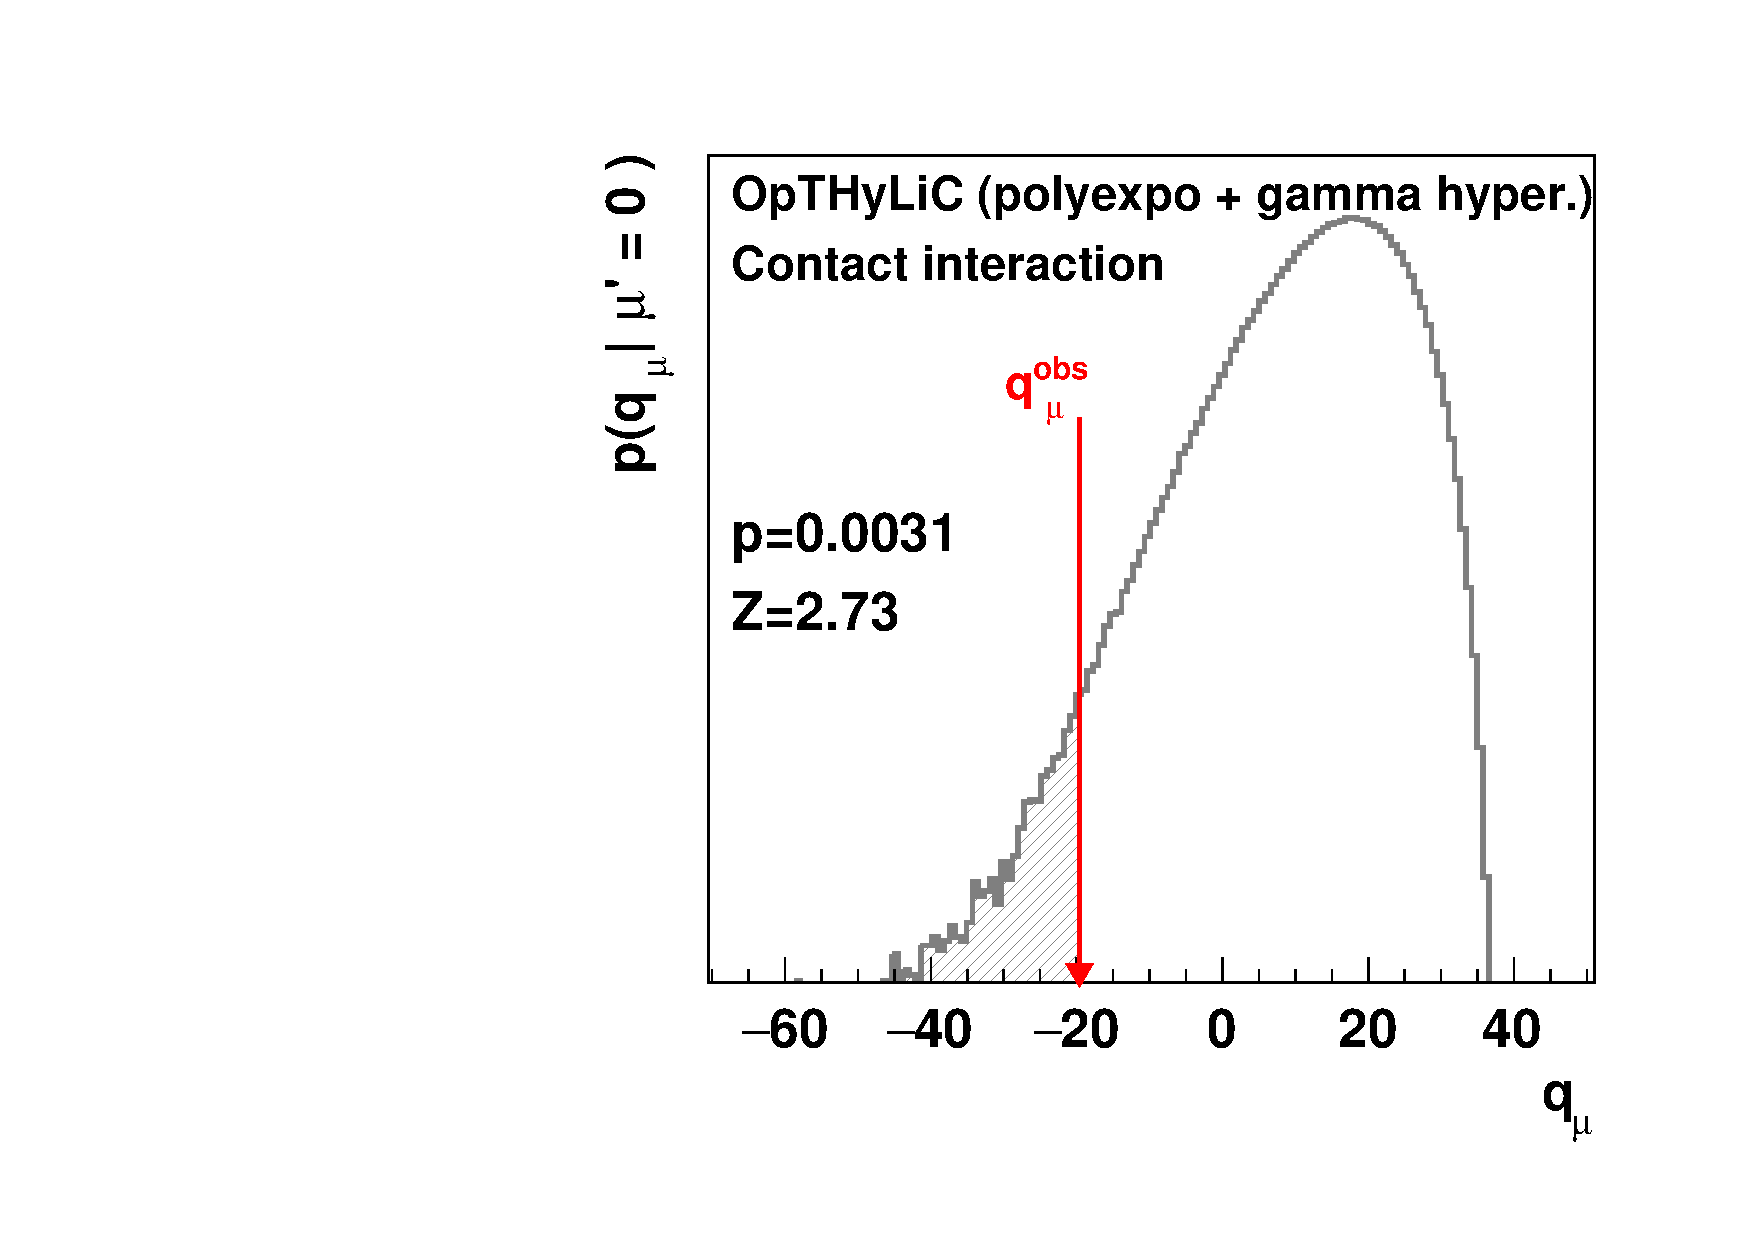
\includegraphics[width=1\textwidth]{Figures/FourTops/significanceContactInteractionPolyExpoGammaHyper.pdf}
\end{figure}
\end{center}
\end{column}
\end{columns}

%$\rightarrow$ Variations d'environ $10\%$

%\textcolor{red}{mettre plot et valeur significance}
%\end{center}
\end{frame}

\begin{frame}
\frametitle{Interpr\'etation bayésienne}

\vspace*{-.2cm}
\begin{small}
\[f\left(\mu|\{\nc\}\right)\propto \displaystyle\int P\left(\{\nc\}|\textcolor{blue}{\mu},\textcolor{red}{\nu}\right)\underbrace{\pi_\nu\left(\nu\right)\pi_\mu\left(\mu\right)}_{priors}\dd\textcolor{red}{\nu}\]

\vspace*{-2.4cm}

\begin{columns}
\begin{column}{0.6\textwidth}
\begin{footnotesize}
\begin{maliste}
\item Configuration
\begin{itemize}
\item Incertitudes stat. : prior normal
\item Interpolation polynomiale + extrapolation exponentielle
\item $\pi(\mu)=\text{constant}$
\end{itemize}
\vspace*{0.1cm}
\item Limite attendue : dataset asimov
\end{maliste}
\end{footnotesize}
\end{column}
\begin{column}{0.5\textwidth}
\hspace*{-2.1cm}
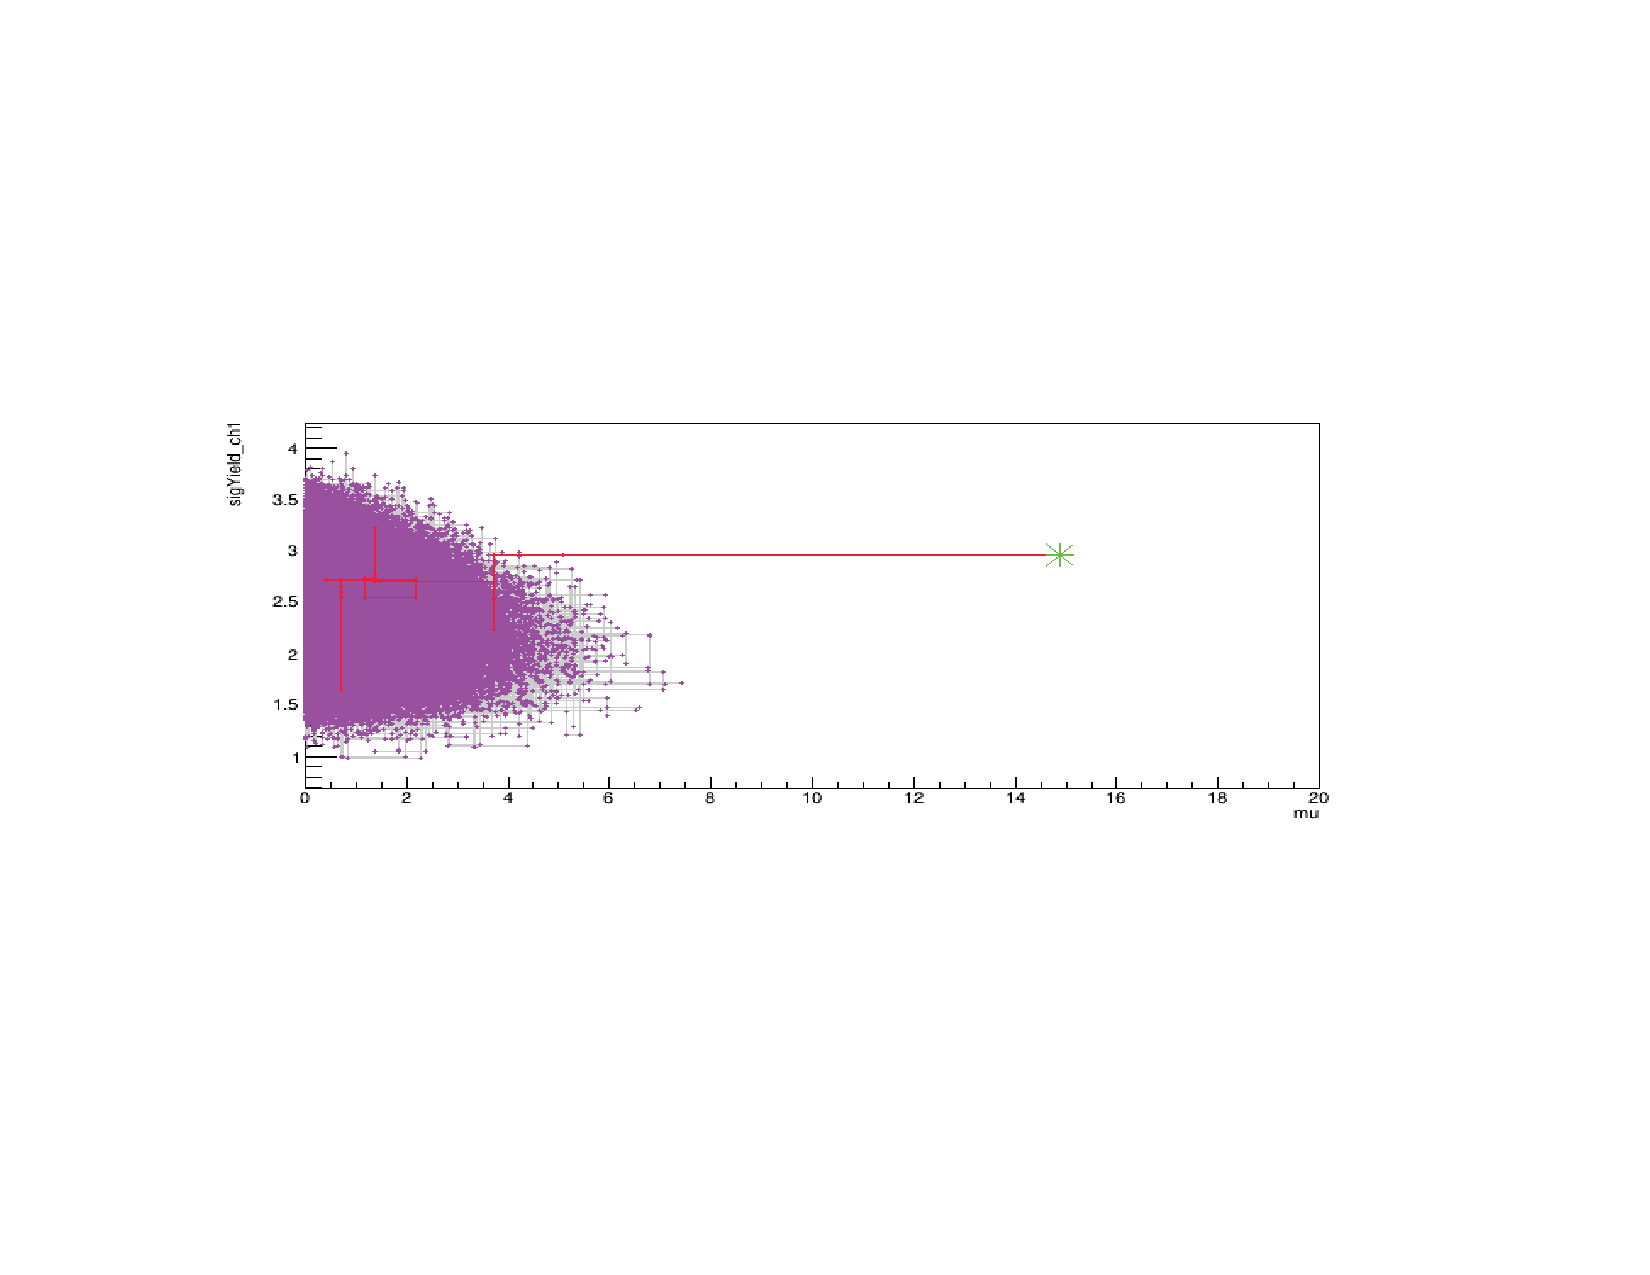
\includegraphics[width=1.75\linewidth]{Figures/FourTops/markovchainexample.pdf}
\end{column}
\end{columns}
\end{small}

\vspace*{-2.5cm}
\begin{figure}[!htb]
\begin{center}
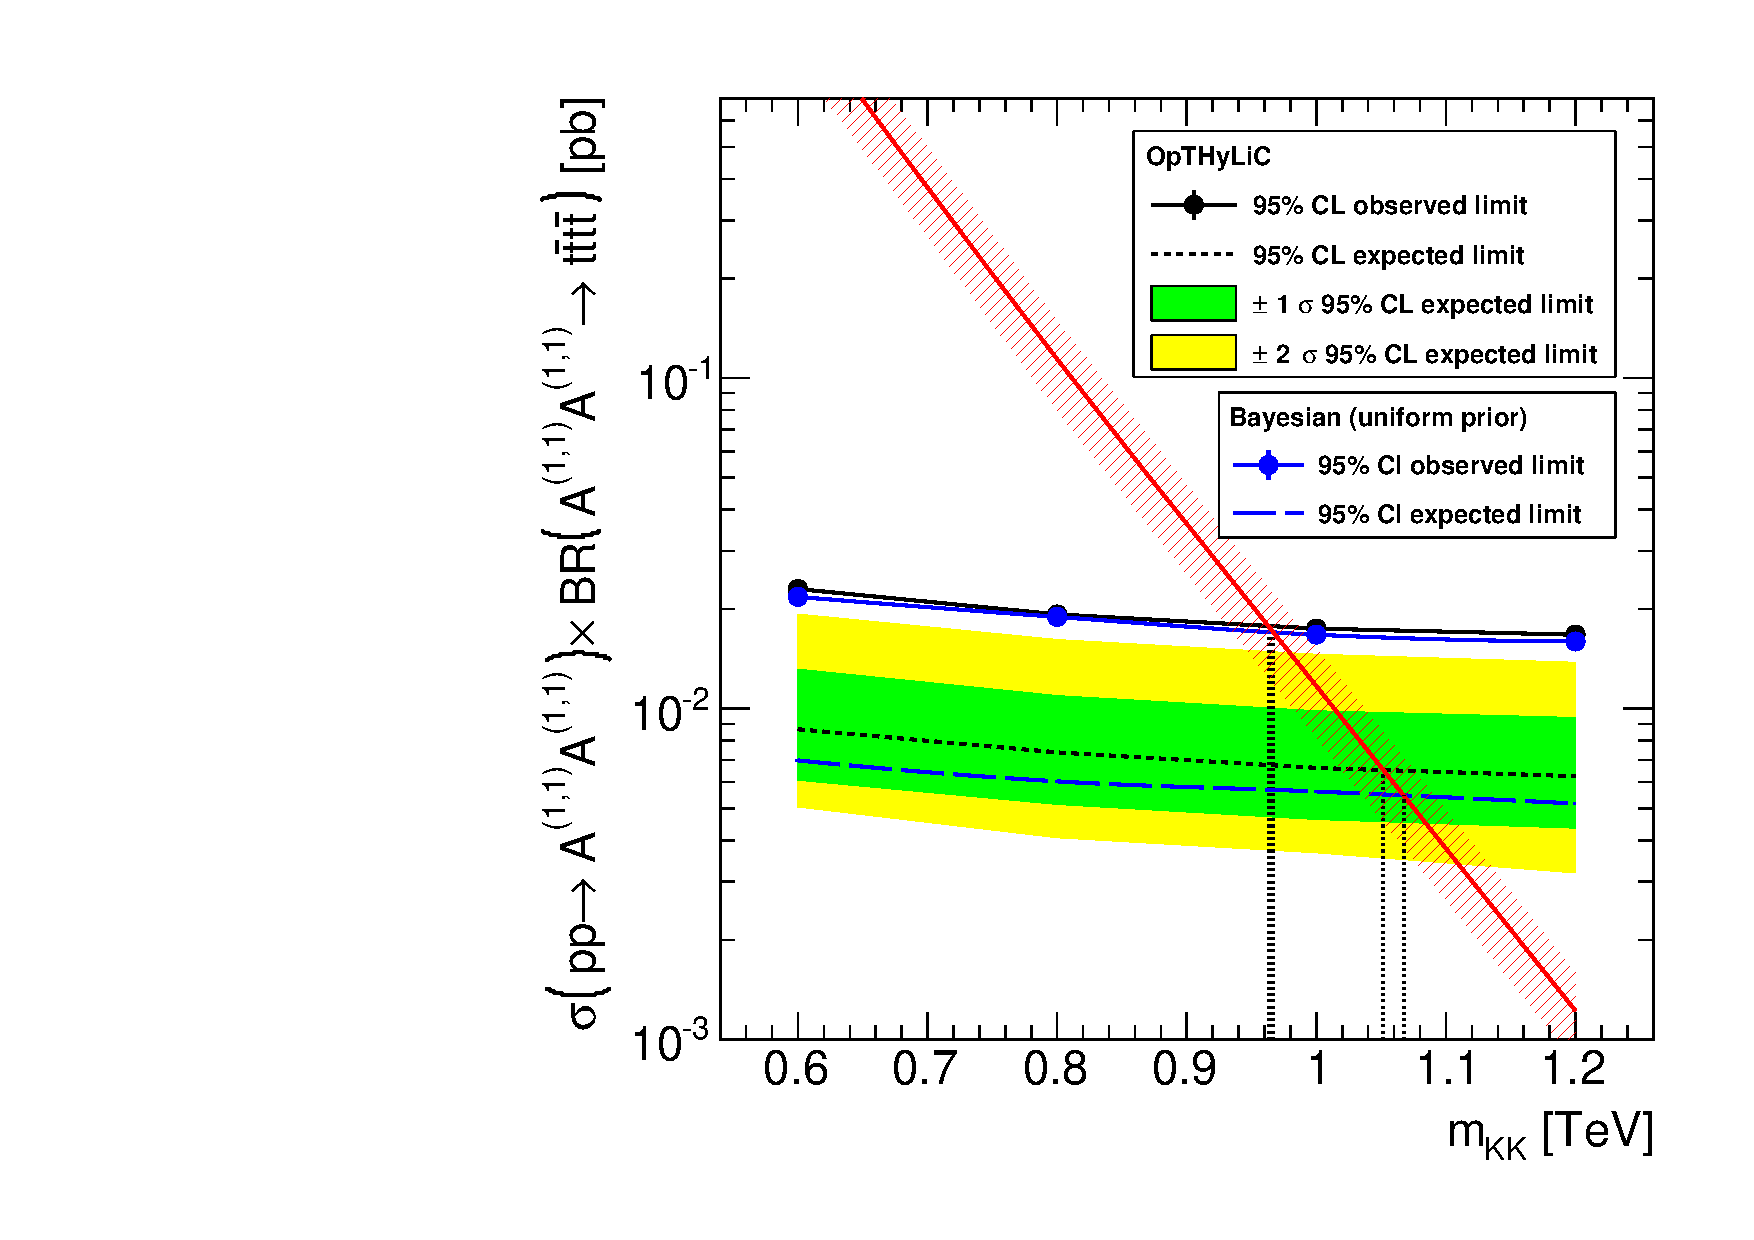
\includegraphics[width=0.38\linewidth]{Figures/FourTops/ExclusionPlot_RPPFullStat_OTHVsBayesian.pdf}
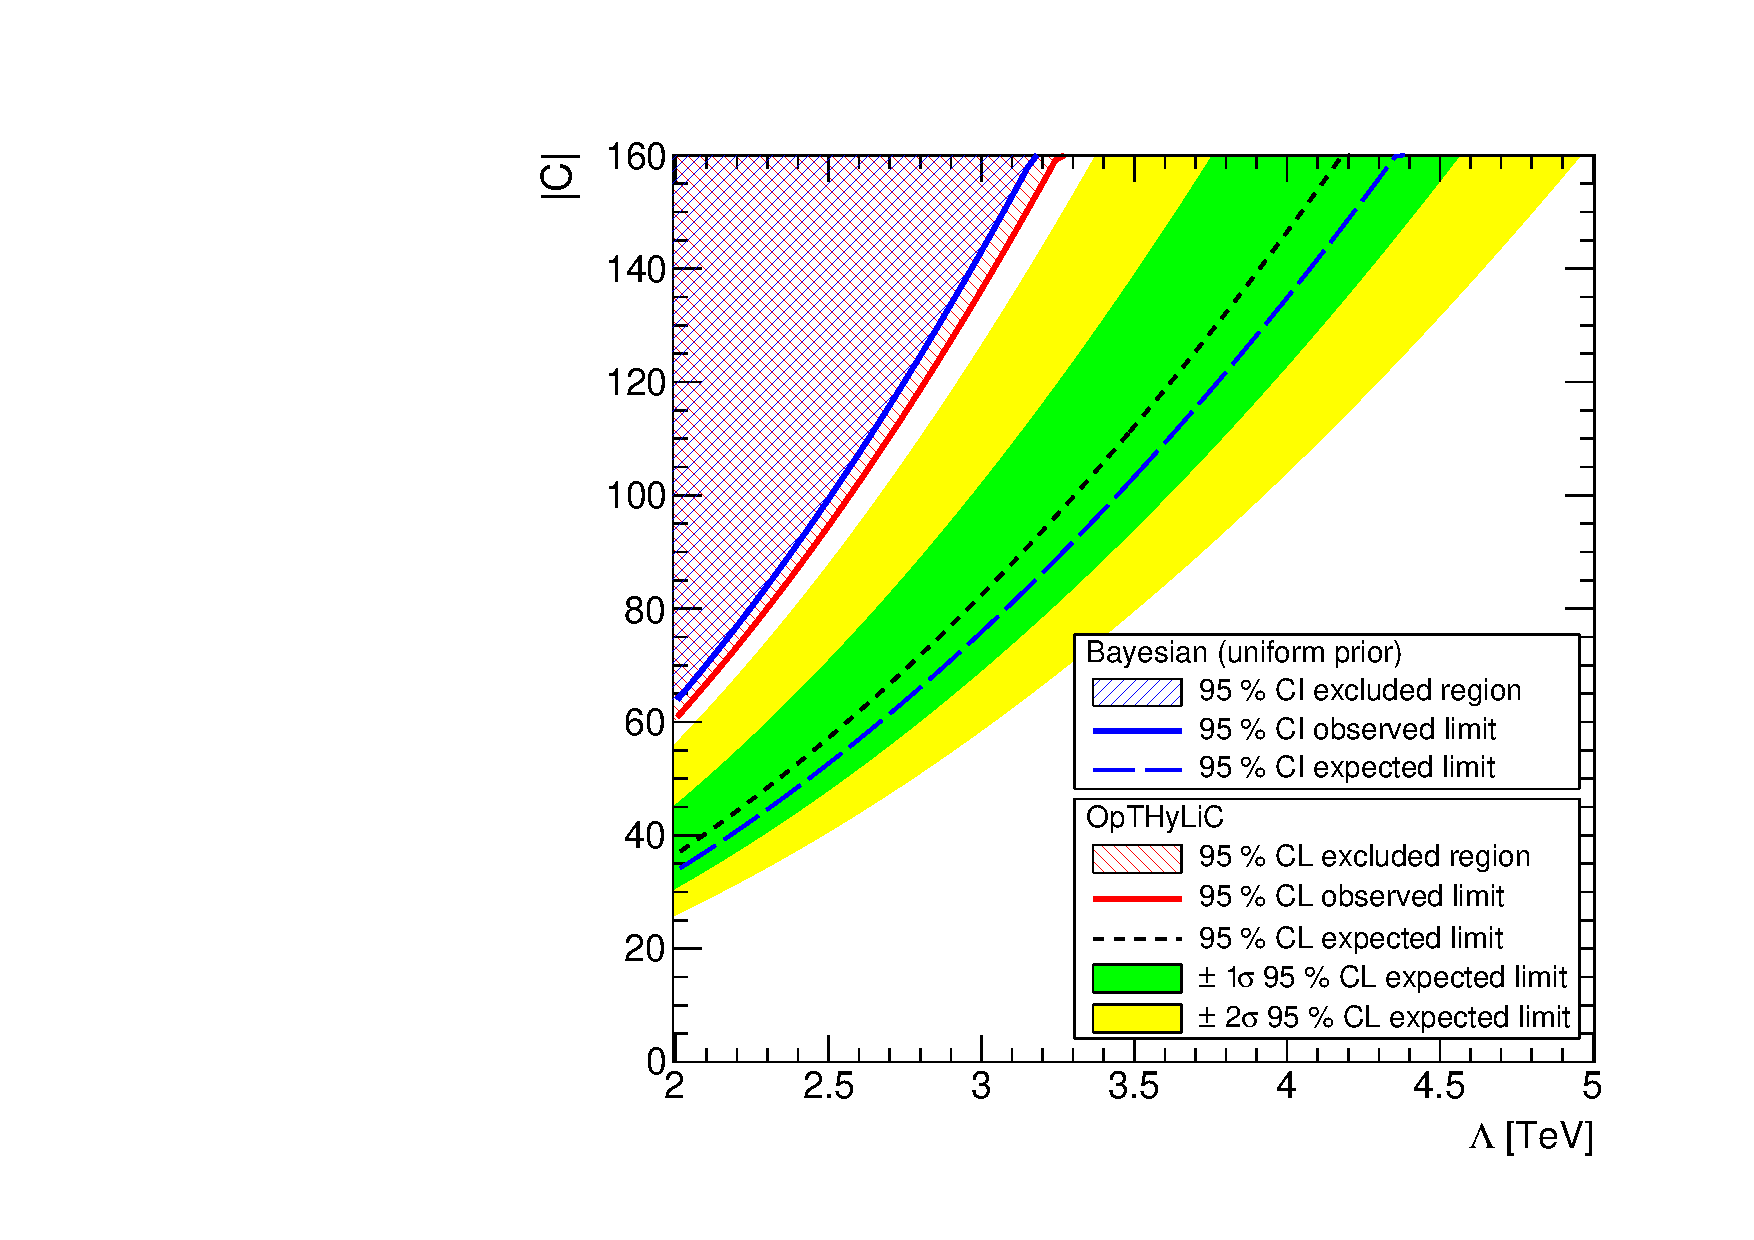
\includegraphics[width=0.4\linewidth]{Figures/FourTops/CVsLambdaForContactInteractionHybridVsBayesian.pdf}
\end{center}
\end{figure}

\end{frame}

\begin{frame}
\frametitle{Interpr\'etation fréquentiste}
\begin{small}
\vspace*{-0.5cm}
\[
\hspace*{-0.5cm}
P(\{\nc\},\{a_j\}|\textcolor{blue}{\mu},\textcolor{red}{\nu})=\prod\limits_c\frac{\left(\textcolor{blue}{\mu} \scc(\textcolor{red}{\nu_j})+\bc(\textcolor{red}{\nu_j})\right)^{\nc}}{\nc!}e^{-\left(\textcolor{blue}{\mu} \scc(\textcolor{red}{\nu_j})+\bc(\textcolor{red}{\nu_j})\right)} \prod_j P_j\left(a_j|\textcolor{red}{\nu_j}\right)\]
\end{small}

\begin{columns}
\begin{column}{0.6\textwidth}
\begin{footnotesize}
\begin{maliste}
%\item Outils utilisés : \histfactory+\roostats
%\vspace*{0.1cm}
\item Exp\'eriences auxilliaires :
\begin{itemize}
\item syst\'ematiques : gaussiennes
\item statistiques : poissonniennes\\
$\rightarrow$ version ``lite''\\
\end{itemize}
%$\rightarrow$ validée dans cas simplifié
\vspace*{0.1cm}
\item Limite asymptotique valide \`a \\quelques \%
\vspace*{0.1cm}
\item Limites attendues à $N\sigma$: $\Est{\mu}=\mu'+N\sigma$
\end{maliste}
\end{footnotesize}
\end{column}
\begin{column}{0.4\textwidth}
\begin{figure}[!htb]
\hspace*{-2.2cm}
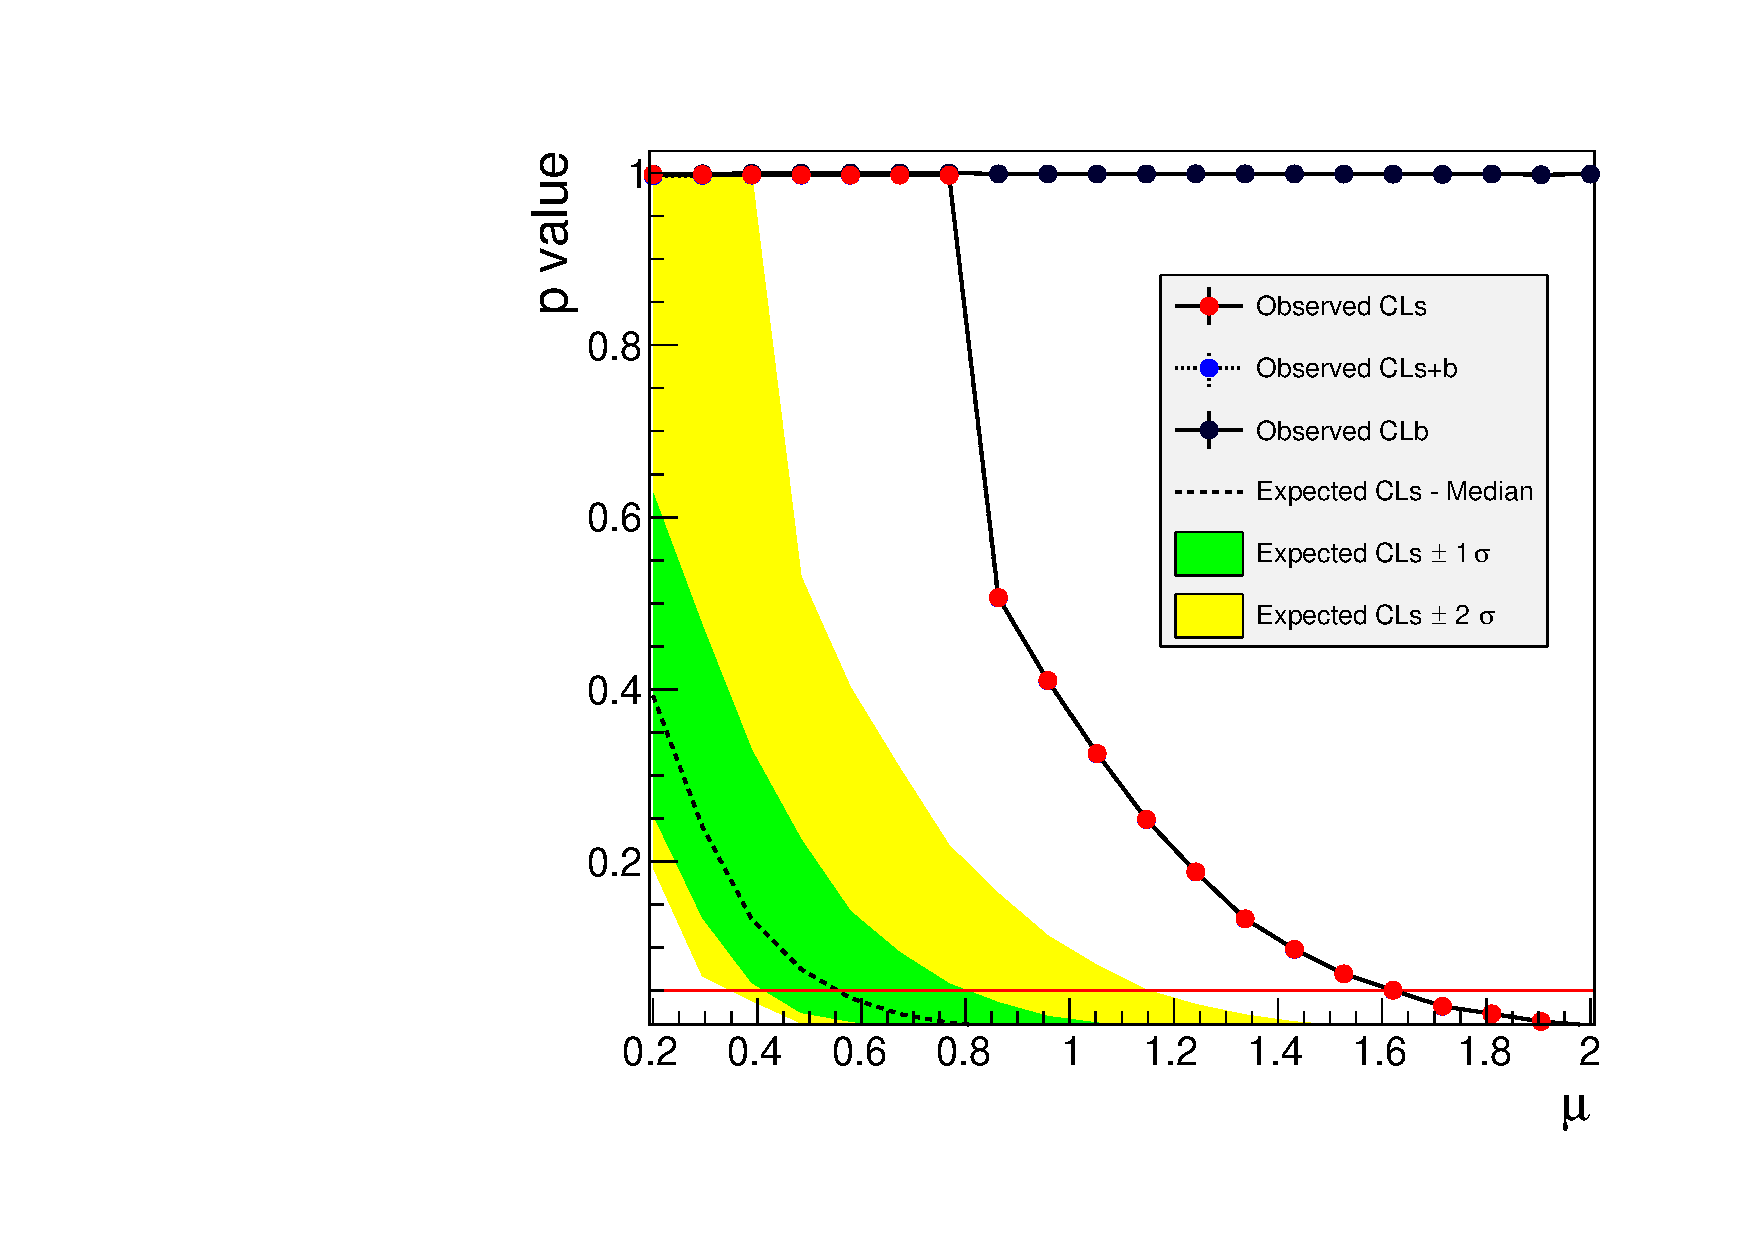
\includegraphics[width=0.62\linewidth]{Figures/FourTops/pureFrequentistmKK1000GeVScan.pdf}\\
\vspace*{-3.4cm}
\hspace*{1.3cm}
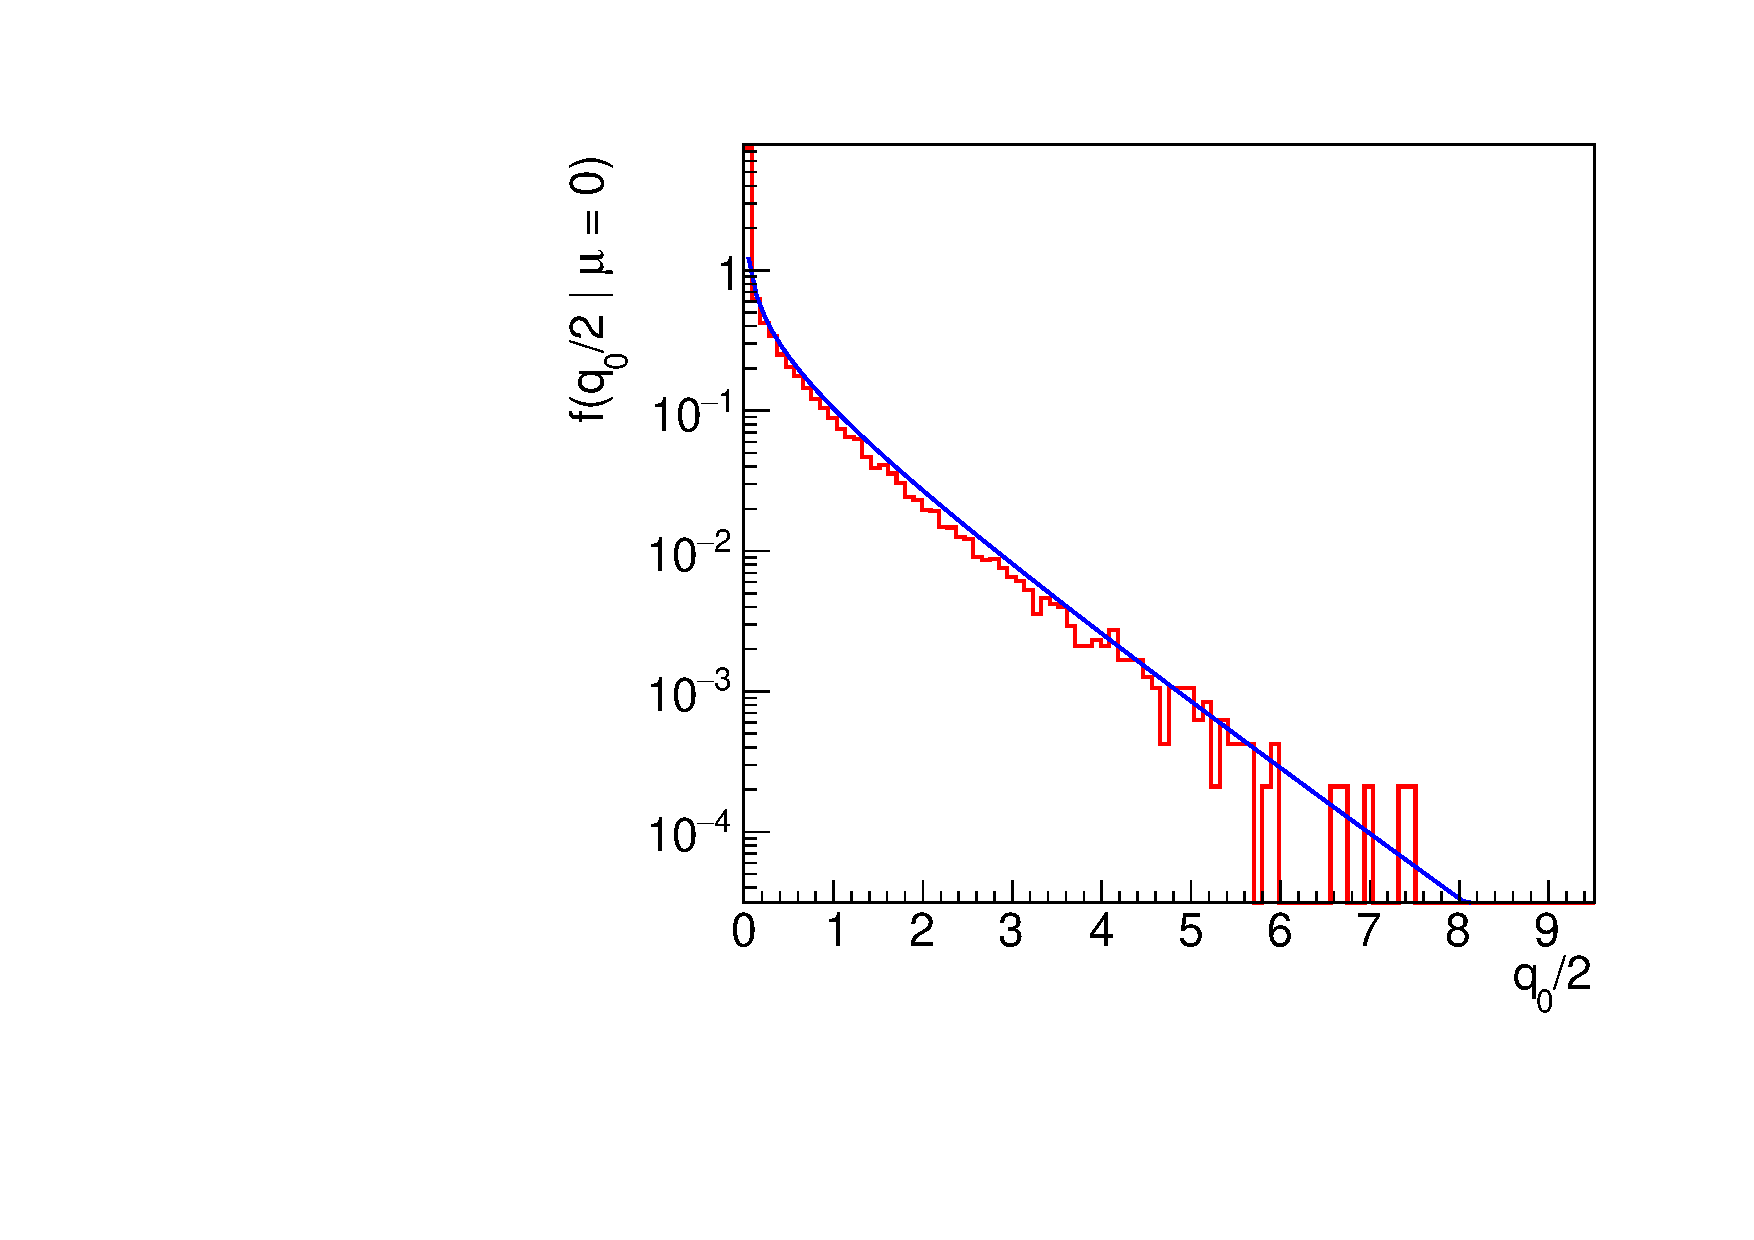
\includegraphics[width=0.76\linewidth]{Figures/FourTops/outputObservationSignificance2UEDRPPmKK1000GeV.pdf}
\put(-70,65){\tiny{2UED/RPP}}
\put(-70,58){\tiny{$m_{KK}=1000$~GeV}}
\end{figure}
\end{column}
\end{columns}

%\vspace*{0.2cm}
\begin{figure}[!htb]
\begin{center}
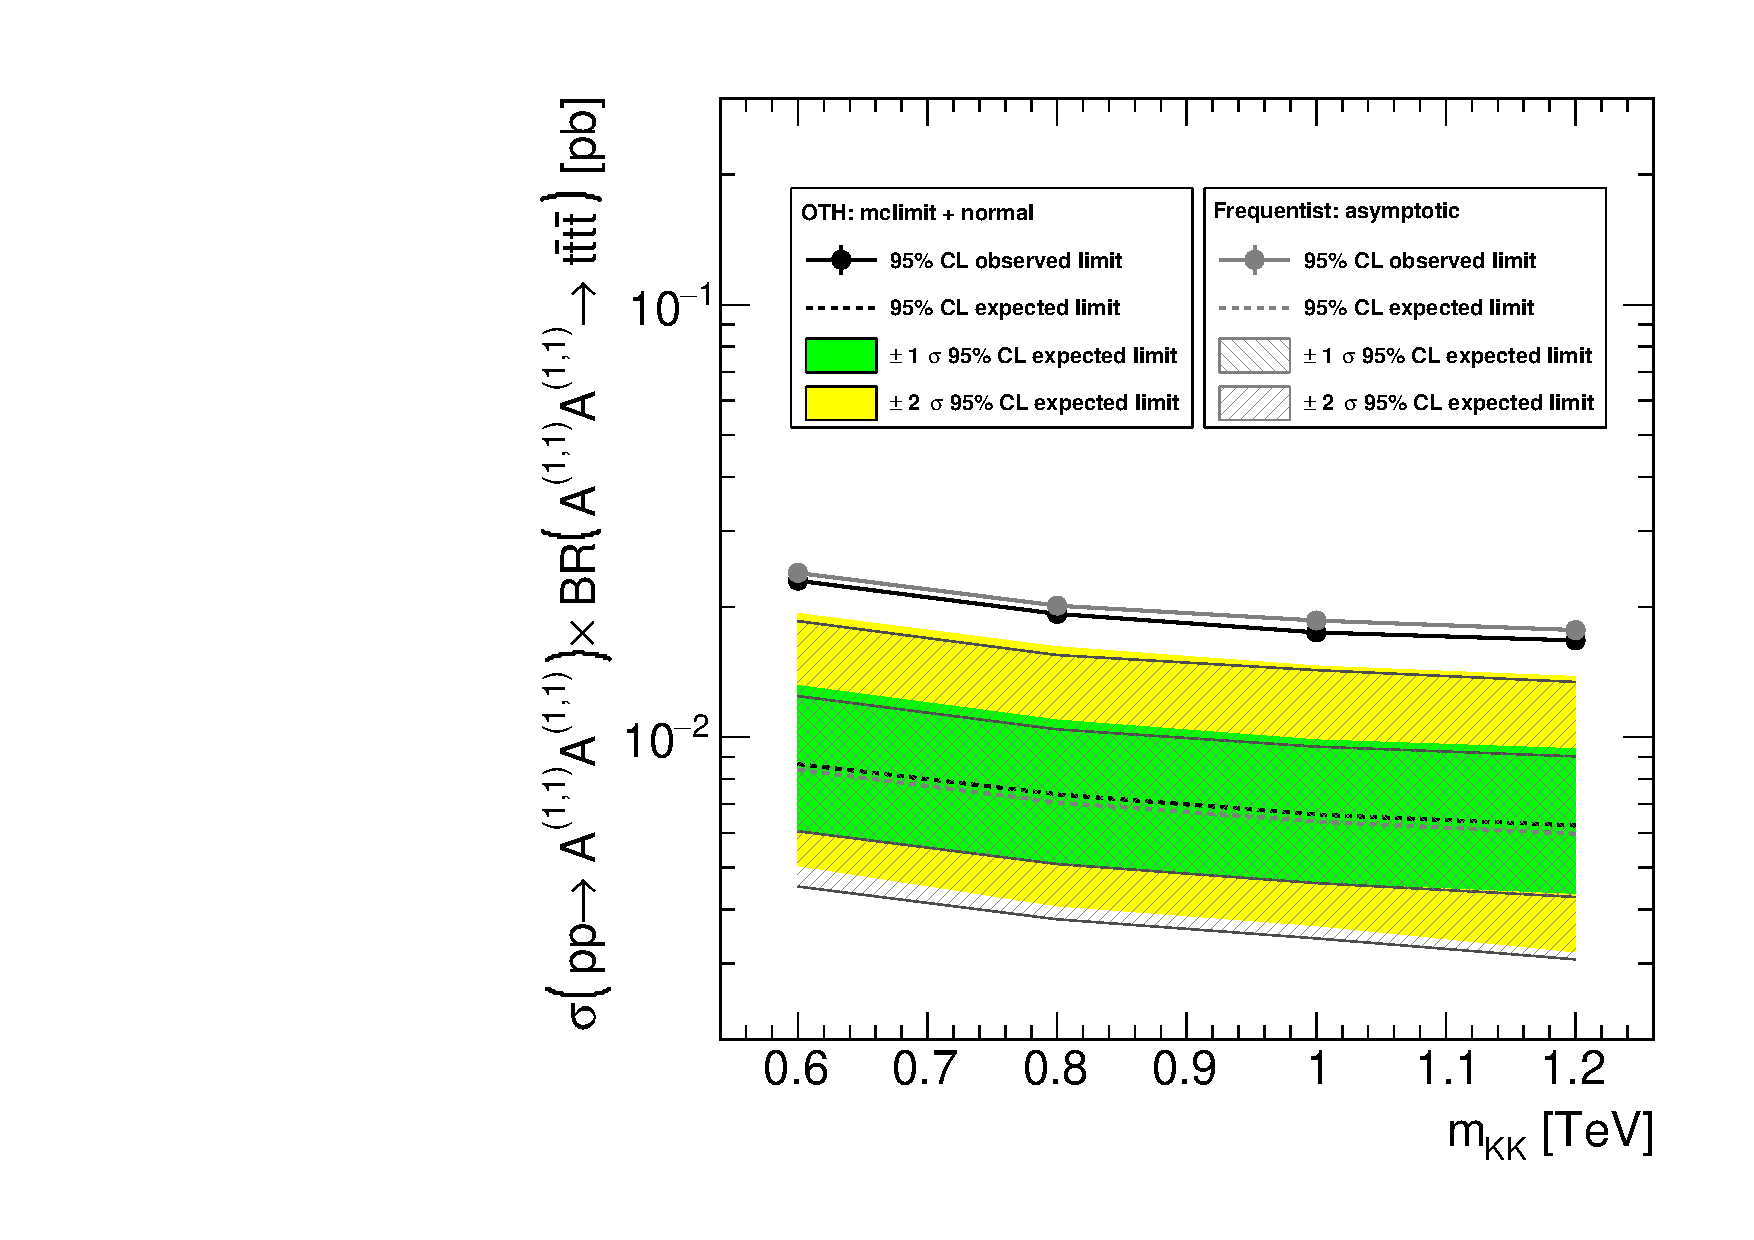
\includegraphics[width=0.32\linewidth]{Figures/FourTops/ExclusionPlot_RPPFullStat_McLimitVsAsymptotic.pdf}
\hspace*{0.2cm}
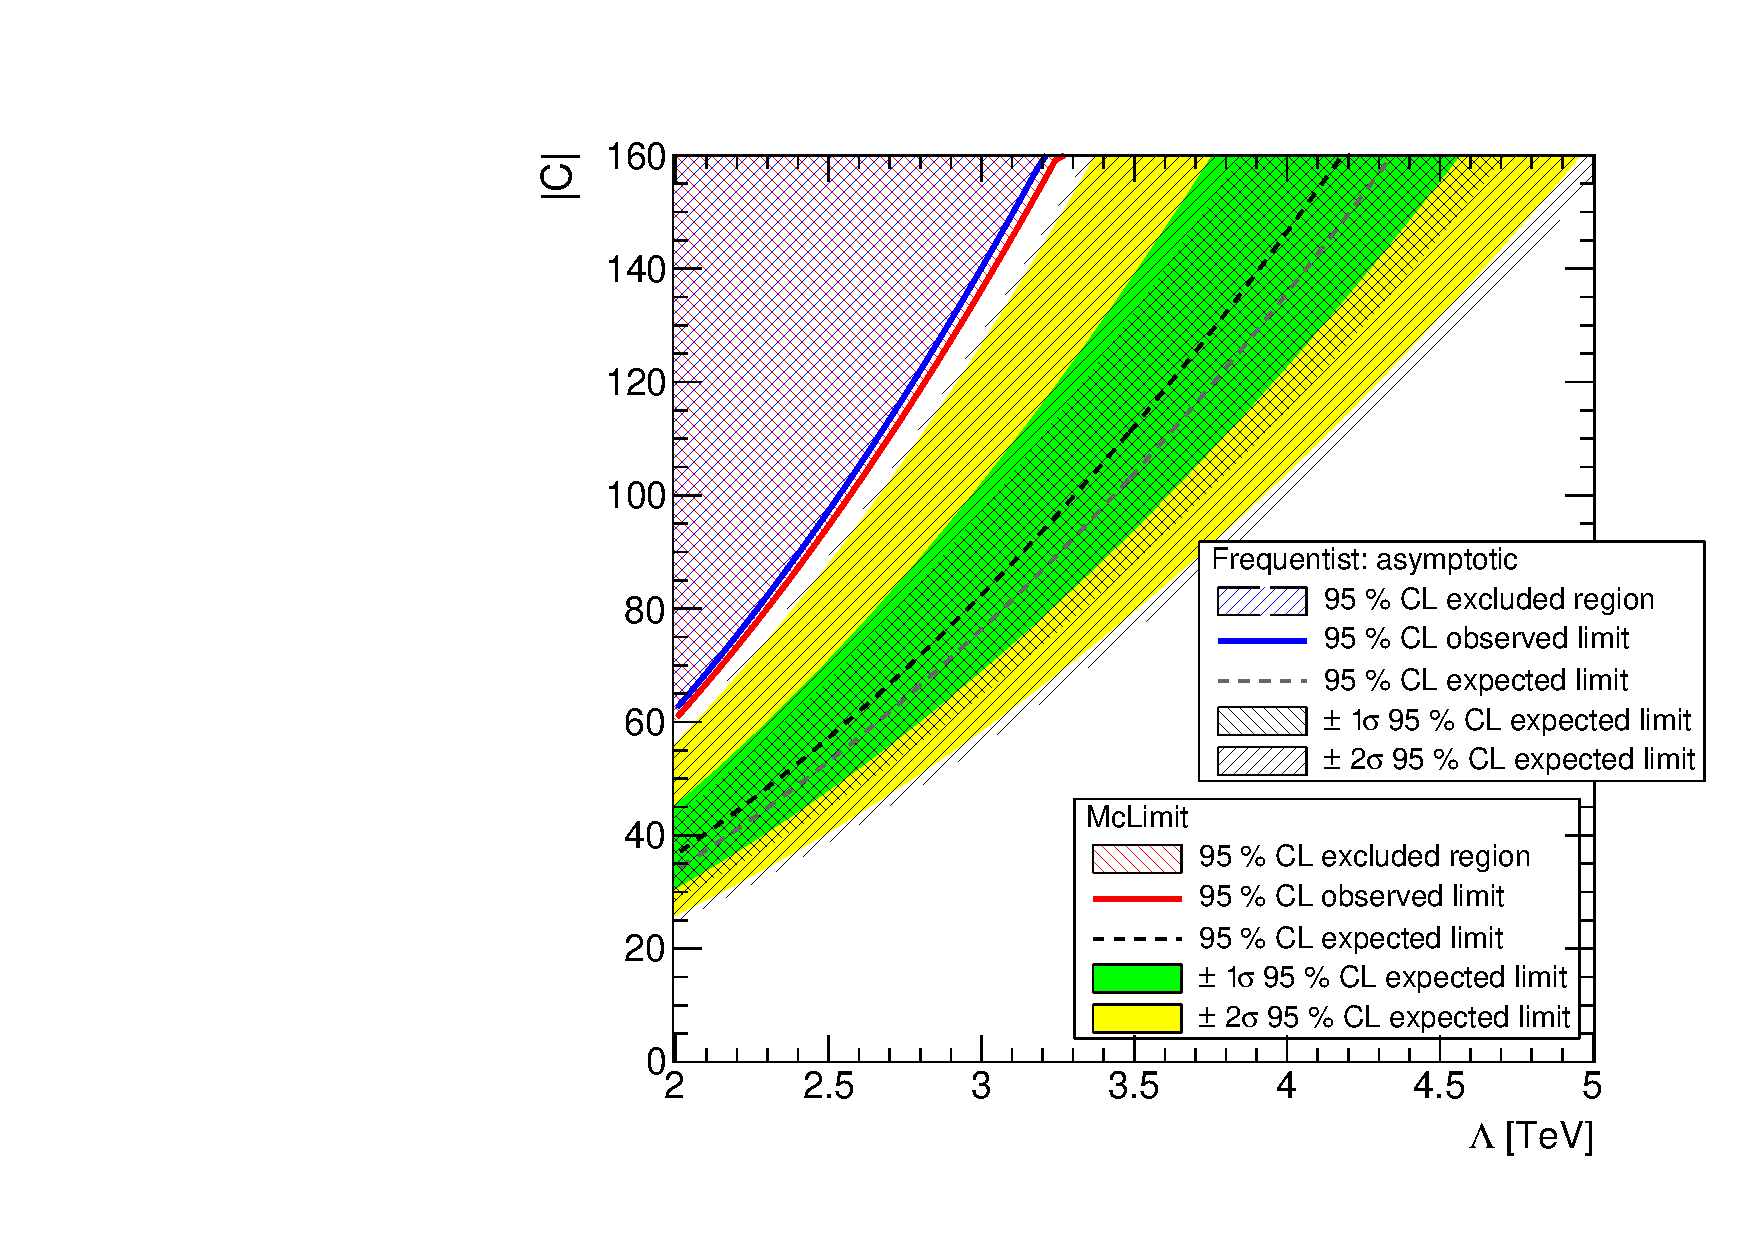
\includegraphics[width=0.34\linewidth]{Figures/FourTops/CVsLambdaForContactInteractionHybridVsAsymptotic.pdf}
\end{center}
\end{figure}

%\begin{scriptsize}
%\begin{table}[!htb]
%  \begin{center}
%    \begin{tabular}{|c|c|c|c|c|c|c|}
%      \cline{2-7}
%      \multicolumn{1}{c|}{} & \multicolumn{6}{c|}{Limites 2UED/RPP $m_{KK}=1000$~GeV}       \\ \cline{2-7}
%      \multicolumn{1}{c|}{}  & $-2\sigma$   & $-1\sigma$  & m\'ediane  & $+1\sigma$  & $+2\sigma$ & observée  \\ \hline
%      calcul exact  &  0,29  &  0,39 & 0,55  & 0,81 & 1,22 &  1,60 \\ \hline
%      calcul asymptotique  & 0,32   & 0,41  &  0,55 & 0,80 & 1,15 & 1,62 \\ \hline
%    \end{tabular}
%  \end{center}
%\end{table}
%\end{scriptsize}

\end{frame}

%\begin{frame}
%\frametitle{Limites fréquentistes}

%\begin{maliste}
%\item Comparaison hybride - fr\'equentiste asymptotique
%\vspace*{0.2cm}
%\item Limites attendues à $N\sigma$: $\Est{\mu}=\mu'+N\sigma$
%\end{maliste}

%\begin{figure}[!htb]
%\begin{center}
%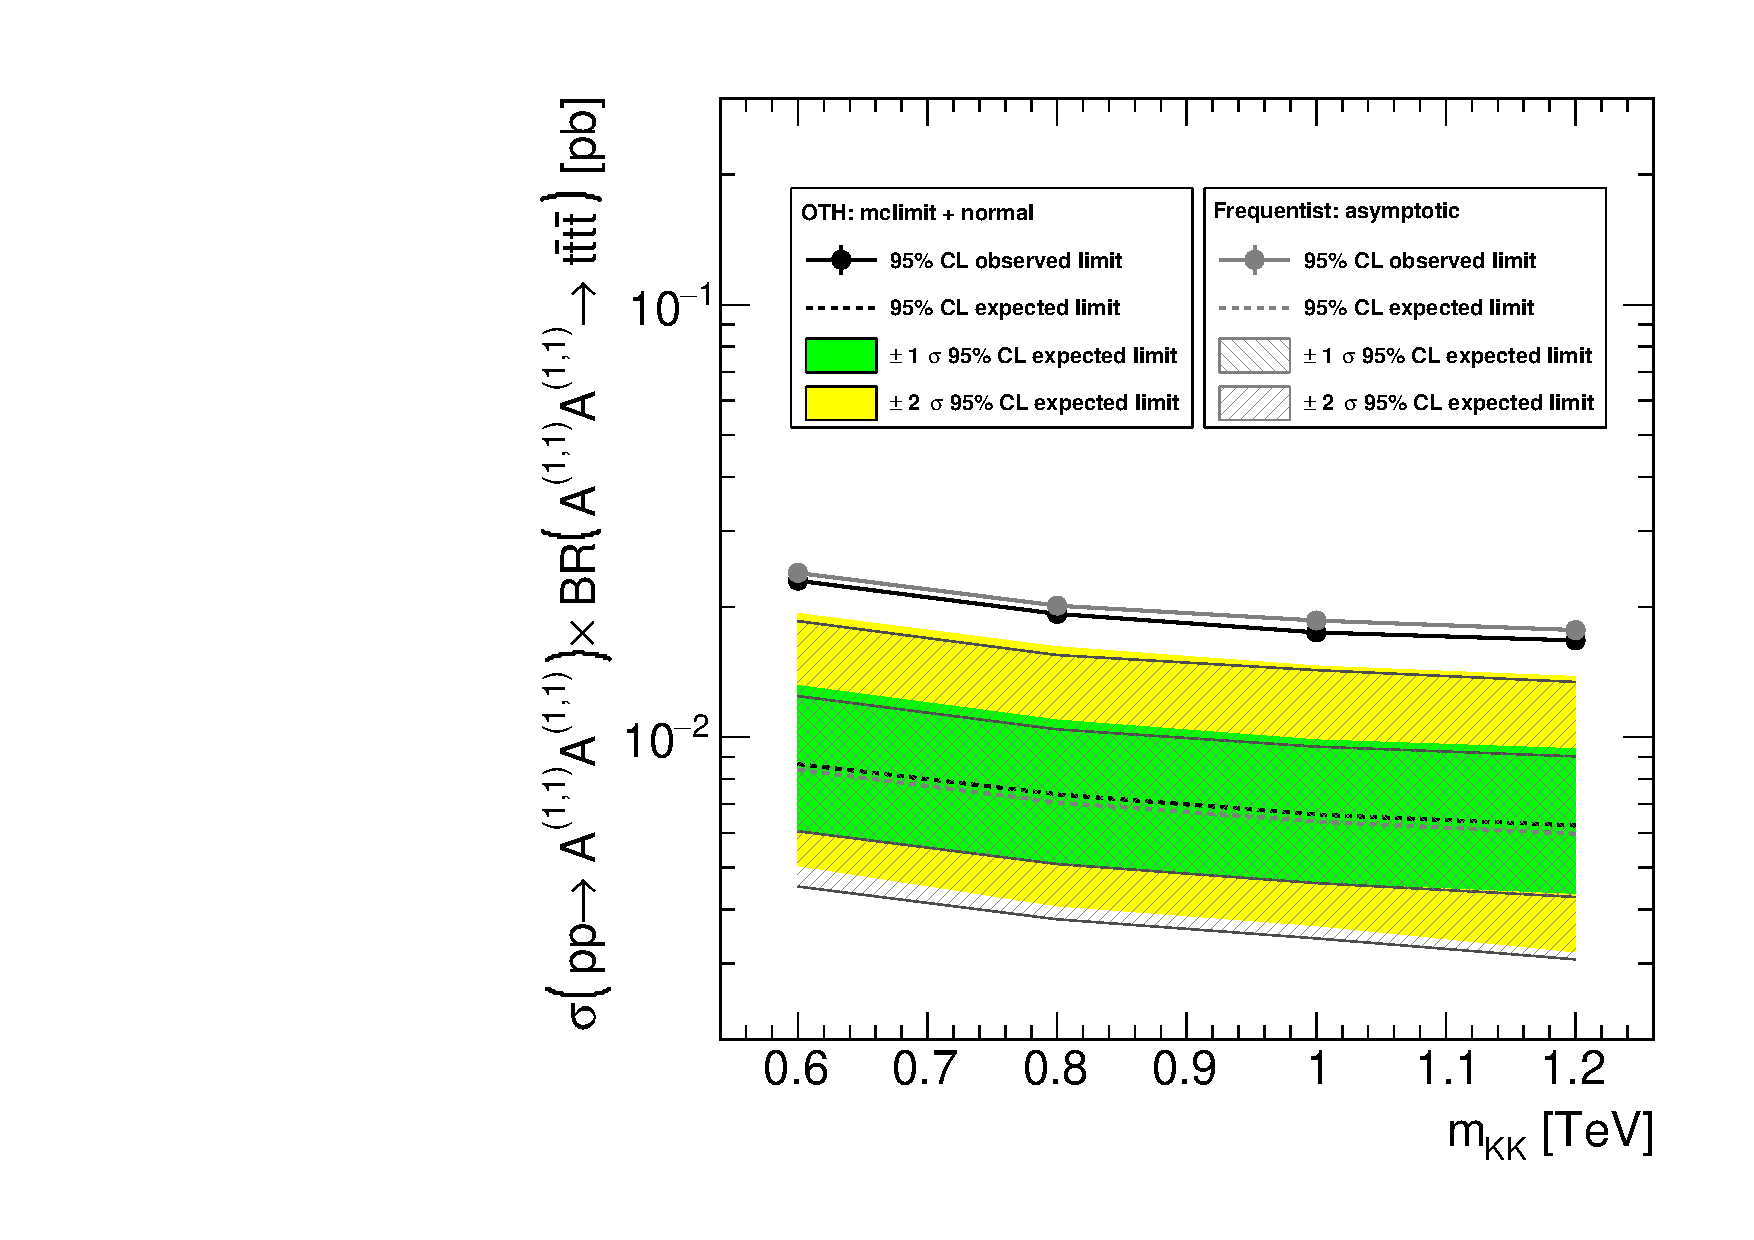
\includegraphics[width=0.45\linewidth]{Figures/FourTops/ExclusionPlot_RPPFullStat_McLimitVsAsymptotic.pdf}
%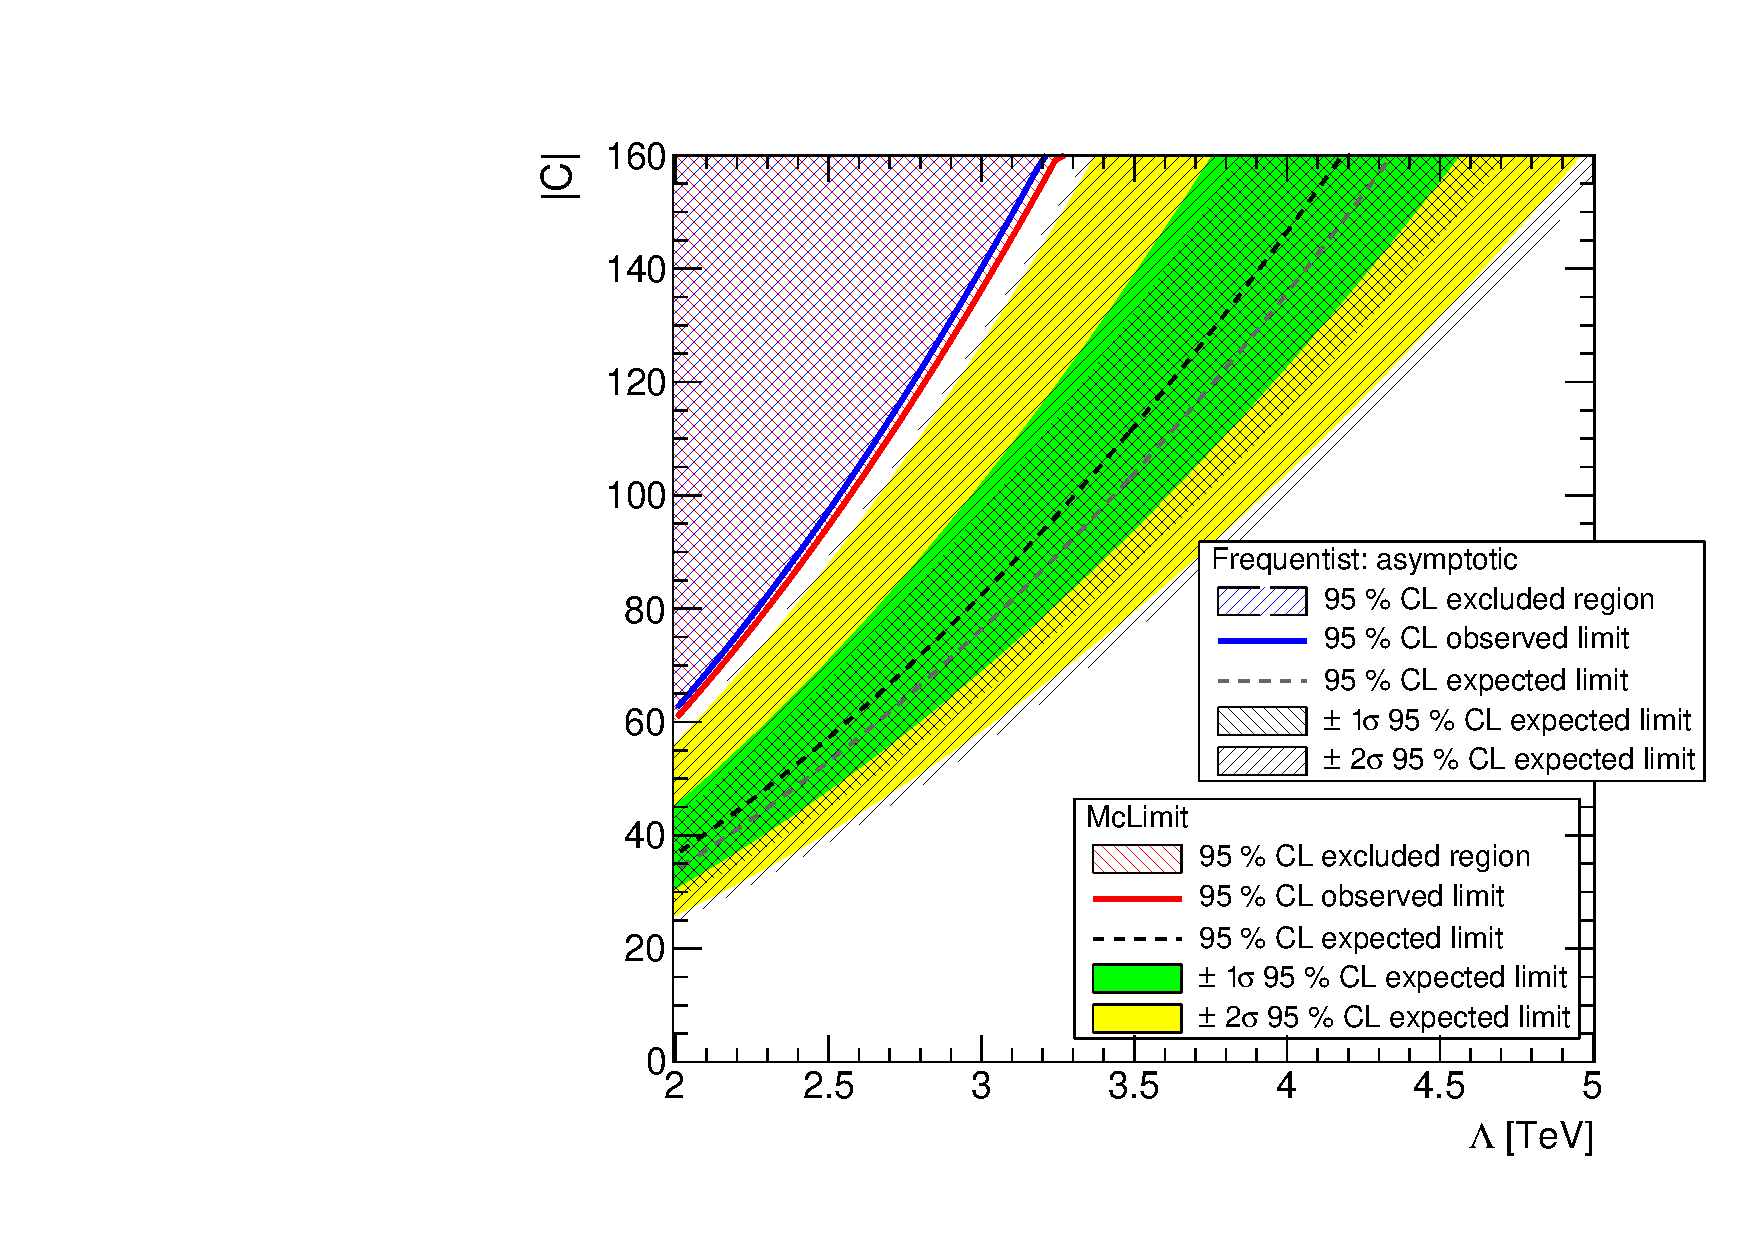
\includegraphics[width=0.47\linewidth]{Figures/FourTops/CVsLambdaForContactInteractionHybridVsAsymptotic.pdf}
%\end{center}
%\end{figure}

%Dire quelque chose sur le fit des paramètres de nuisance ? (cas conditionnel/non-conditionnel)

%\begin{center}
%$\rightarrow$ Variations $< 10$ \%
%\end{center}

%\begin{maliste}
%\item \textcolor{magenta}{Conclusion g\'en\'erale : limites et significances valid\'ees \`a $\sim 10\%$ pr\`es}
%\end{maliste}

%\end{frame}

\begin{comment}
\begin{frame}
\frametitle{Conclusion}

\begin{maliste}
\item Diff\'erences entre limites observ\'ees sur sections efficaces :
\begin{itemize}
\item hybride (d\'efault) - hybride (vari\'ee) $< 10\%$
\item hybride (d\'efault) - bay\'esien $<8\%$
\item hybride (d\'efault) - fr\'equentiste $<7\%$
\end{itemize}
\vspace*{0.1cm}
\begin{center}
$\rightarrow$ Limites observ\'ees sur sections efficaces valid\'ees \`a $\sim 10\%$
\end{center}
\item Diff\'erences entre limites observ\'ees sur $m_{KK} < 20~$GeV
\vspace*{0.1cm}
\item Premi\`eres limites sur processus 4 tops mod\`ele standard, interaction contact
\item 
\item \textcolor{red}{Conclusion g\'en\'erale}
\end{maliste}

%\begin{footnotesize}
%\begin{table}[!htb]
%  \begin{center}
%    \scalebox{0.9}{    
%      \begin{tabular}{|c|c|c|c|c|}
%        \hline
%        \multirow{3}{*}{Signal} & \multicolumn{4}{c|}{Limite observ\'ee (fb)} \\ \cline{2-5}
% &   hybride  & hybride   &   \multirow{2}{*}{bayes}  &   \multirow{2}{*}{fr\'eq}   \\ 
% & d\'efault  & vari\'ee  & & \\ \hline
%2UED/RPP $m_{KK}=600$ GeV  &   23.0    & 24.5 (+6.5\%)    &   21.8 (-5.2\%)    &    24.0 (+4.3\%)   \\ \hline
%2UED/RPP $m_{KK}=800$ GeV  &   19.3    & 20.6 (+6.7\%)    &   19.0 (-1.6\%)    &    20.1 (+4.1\%)   \\ \hline 
%2UED/RPP $m_{KK}=1000$ GeV &   17.5    & 18.7 (+6.9\%)    &   16.7 (-4.6\%)    &    18.6 (+6.3\%)   \\ \hline  
%2UED/RPP $m_{KK}=1200$ GeV &   16.7    & 17.8 (+6.6\%)    &   16.0 (-4.2\%)    &    17.8 (+6.6\%)   \\ \hline  
%Interaction contact       &   61.2    & 67.5 (+10.3\%)   &   66.3 (+8.3\%)    &    64.7 (+5.7\%)   \\ \hline  
%Mod\`ele standard         &   70.1    & 77.1 (+10.0\%)   &   66.7 (-4.9\%)    &    74.4 (+6.1\%)   \\ \hline  
%\end{tabular}
%}
    %\caption{Limites d'exclusion sur la section efficace de production (en fb) pour les diff\'erents signaux consid\'er\'es dans cette analyse. Les limites hybrides (bay\'esiennes) sont calcul\'ees avec le programme \opthylic~\`a 95\% CL (\tifosi~\`a 95\% CI). Les limites bay\'esiennes sont calcul\'ees avec une distribution \prior~uniforme sur le param\`etre d'int\'er\^et. Les limites attendues sont les limites m\'edianes sous l'hypoth\`ese du bruit de fond dans le cas hybride et les limites calcul\'ees avec un échantillon \english{asimov} dans le cas bay\'esien. Pour la production par interaction de contact, les nombres d'\'ev\'enements ont \'et\'e obtenus avec $C/\Lambda^2=-4\pi$~TeV$^{-2}$}\label{tab:comparaisonLimitesHybrideBayesienne}
%\end{center}
%\end{table}
%\end{footnotesize}

\end{frame}
\end{comment}
